\documentclass{beamer}

%Setting theme of beamer
\mode<presentation>{

% The Beamer class comes with a number of default slide themes
% which change the colors and layouts of slides. Below this is a list
% of all the themes, uncomment each in turn to see what they look like.

%\usetheme{default}
%\usetheme{AnnArbor}
%\usetheme{Antibes}
%\usetheme{Bergen}
%\usetheme{Berkeley}
%\usetheme{Berlin}
%\usetheme{Boadilla}
%\usetheme{CambridgeUS}
%\usetheme{Copenhagen}
%\usetheme{Darmstadt}
%\usetheme{Dresden}
%\usetheme{Frankfurt}
%\usetheme{Goettingen}
%\usetheme{Hannover}
%\usetheme{Ilmenau}
%\usetheme{JuanLesPins}
%\usetheme{Luebeck}
\usetheme{Madrid}
%\usetheme{Malmoe}
%\usetheme{Marburg}
%\usetheme{Montpellier}
%\usetheme{PaloAlto}
%\usetheme{Pittsburgh}
%\usetheme{Rochester}
%\usetheme{Singapore}
%\usetheme{Szeged}
%\usetheme{Warsaw}

% As well as themes, the Beamer class has a number of color themes
% for any slide theme. Uncomment each of these in turn to see how it
% changes the colors of your current slide theme.

\usecolortheme{default}
%\usecolortheme{albatross}
%\usecolortheme{beaver}
%\usecolortheme{beetle}
%\usecolortheme{crane}
%\usecolortheme{dolphin}
%\usecolortheme{dove}
%\usecolortheme{fly}
%\usecolortheme{lily}
%\usecolortheme{orchid}
%\usecolortheme{rose}
%\usecolortheme{seagull}
%\usecolortheme{seahorse}
%\usecolortheme{whale}
%\usecolortheme{wolverine}

%\setbeamertemplate{footline} % To remove the footer line in all slides uncomment this line
%\setbeamertemplate{footline}[frame number] % To replace the footer line in all slides with a simple slide count uncomment this line

%\setbeamertemplate{navigation symbols}{} % To remove the navigation symbols from the bottom of all slides uncomment this line

\setbeamercovered{transparent}

%\usefonttheme{serif}

%\newcommand*\oldmacro{}%
%\let\oldmacro\insertshorttitle%
%\renewcommand*\insertshorttitle{%
  %\oldmacro\hfill%
  %\insertframenumber\,/\,\inserttotalframenumber}

\setbeamertemplate{caption}[numbered]
\setbeamercolor{caption name}{fg=structure!70!black}
}


%Import other required packages, e.g. 'ctex'
\usepackage[T1]{fontenc}        % Encoding
\usepackage[utf8]{inputenc}     % Encoding
\usepackage{multicol}
\usepackage{ctex}               % Support for zh_cn
\usepackage{amsmath}            % Allows math
%\usepackage{newtxtext,newtxmath}
\usepackage{mathptmx}
\usepackage{graphicx}           % Allows including images
\usepackage{wrapfig}            % Images placement require
\usepackage{float}              % Images float
\usepackage{subfigure}          % subplot support
\usepackage{booktabs}           % Allows the use of \toprule, \midrule and \bottomrule in tables
\usepackage{tcolorbox}          % Allows color table
\usepackage{multirow}           % Allows multiple row in table
\usepackage{enumerate}          % Allows enumerate

%\usepackage[linesnumbered,ruled]{algorithm2e} % Allows algorithm
\usepackage{algpseudocode}
%\renewcommand{\algorithmcfname}{算法} % Change 'Algorithm x' to '算法 x'

%-----------------------------------------------------------
%This block of code defines the information to appear in the
%Title page
\title[Master Thesis Defense]
{基于容器的负载预测模型\\
与能耗优化调度策略研究}

\author[ZeTao Wang]
{答辩人:~王泽涛\inst{1} \and 导师:~林伟伟\inst{2}}

\institute[SCUT]
{
    \inst{1}
    华南理工大学\ 计算机科学与工程学院
    \and
    \inst{2}
    华南理工大学\ 计算机科学与工程学院
}

\logo{

\includegraphics[scale=0.2]{figures/logo.jpg}
}

\date[June. 2019]
{2019年6月}
%End of title page configuration
%-----------------------------------------------------------



%-----------------------------------------------------------
%The next block of commands puts the table of contents at the
%beginning of each section and highlights the current section:

\AtBeginSection[]
{
  \begin{frame}
    \frametitle{目录}
    \tableofcontents[currentsection]
  \end{frame}
}
%-----------------------------------------------------------


\begin{document}

%Title of the document
%This next statement create title page
\frame{\titlepage}

%---------------------------------------------------------
%This block of code is for the table of contents after
%the title page
\begin{frame}
\frametitle{目录}
\tableofcontents[hideothersubsections]
\end{frame}
%---------------------------------------------------------

%Background
%Title of section
\section{问题背景}

\begin{frame}
\frametitle{问题背景}
\begin{itemize}
    \item<1-> 虚拟机和容器
    \begin{itemize}
        \item<1-> 虚拟机:Hypervisor
        \item<1-> 容器:Namespace和CGgroups
    \end{itemize}
    \item<2-> 云计算运行模式:IaaS,PaaS和SaaS转变到CaaS
    \begin{itemize}
        \item<2-> \color{green}{容器简单部署和快速可用}
        \item<2-> \color{gray}{\sout{安全问题}}
        \item<2-> \color{gray}{\sout{资源抢占}}
        \item<2-> \color{blue}{\checkmark CaaS性能损耗低}
    \end{itemize}
    \item<3-> 能耗优化与绿色计算
\end{itemize}

\begin{figure}[htb]
\visible<1->{
    \centering
    \begin{minipage}{130pt}
    \centering
    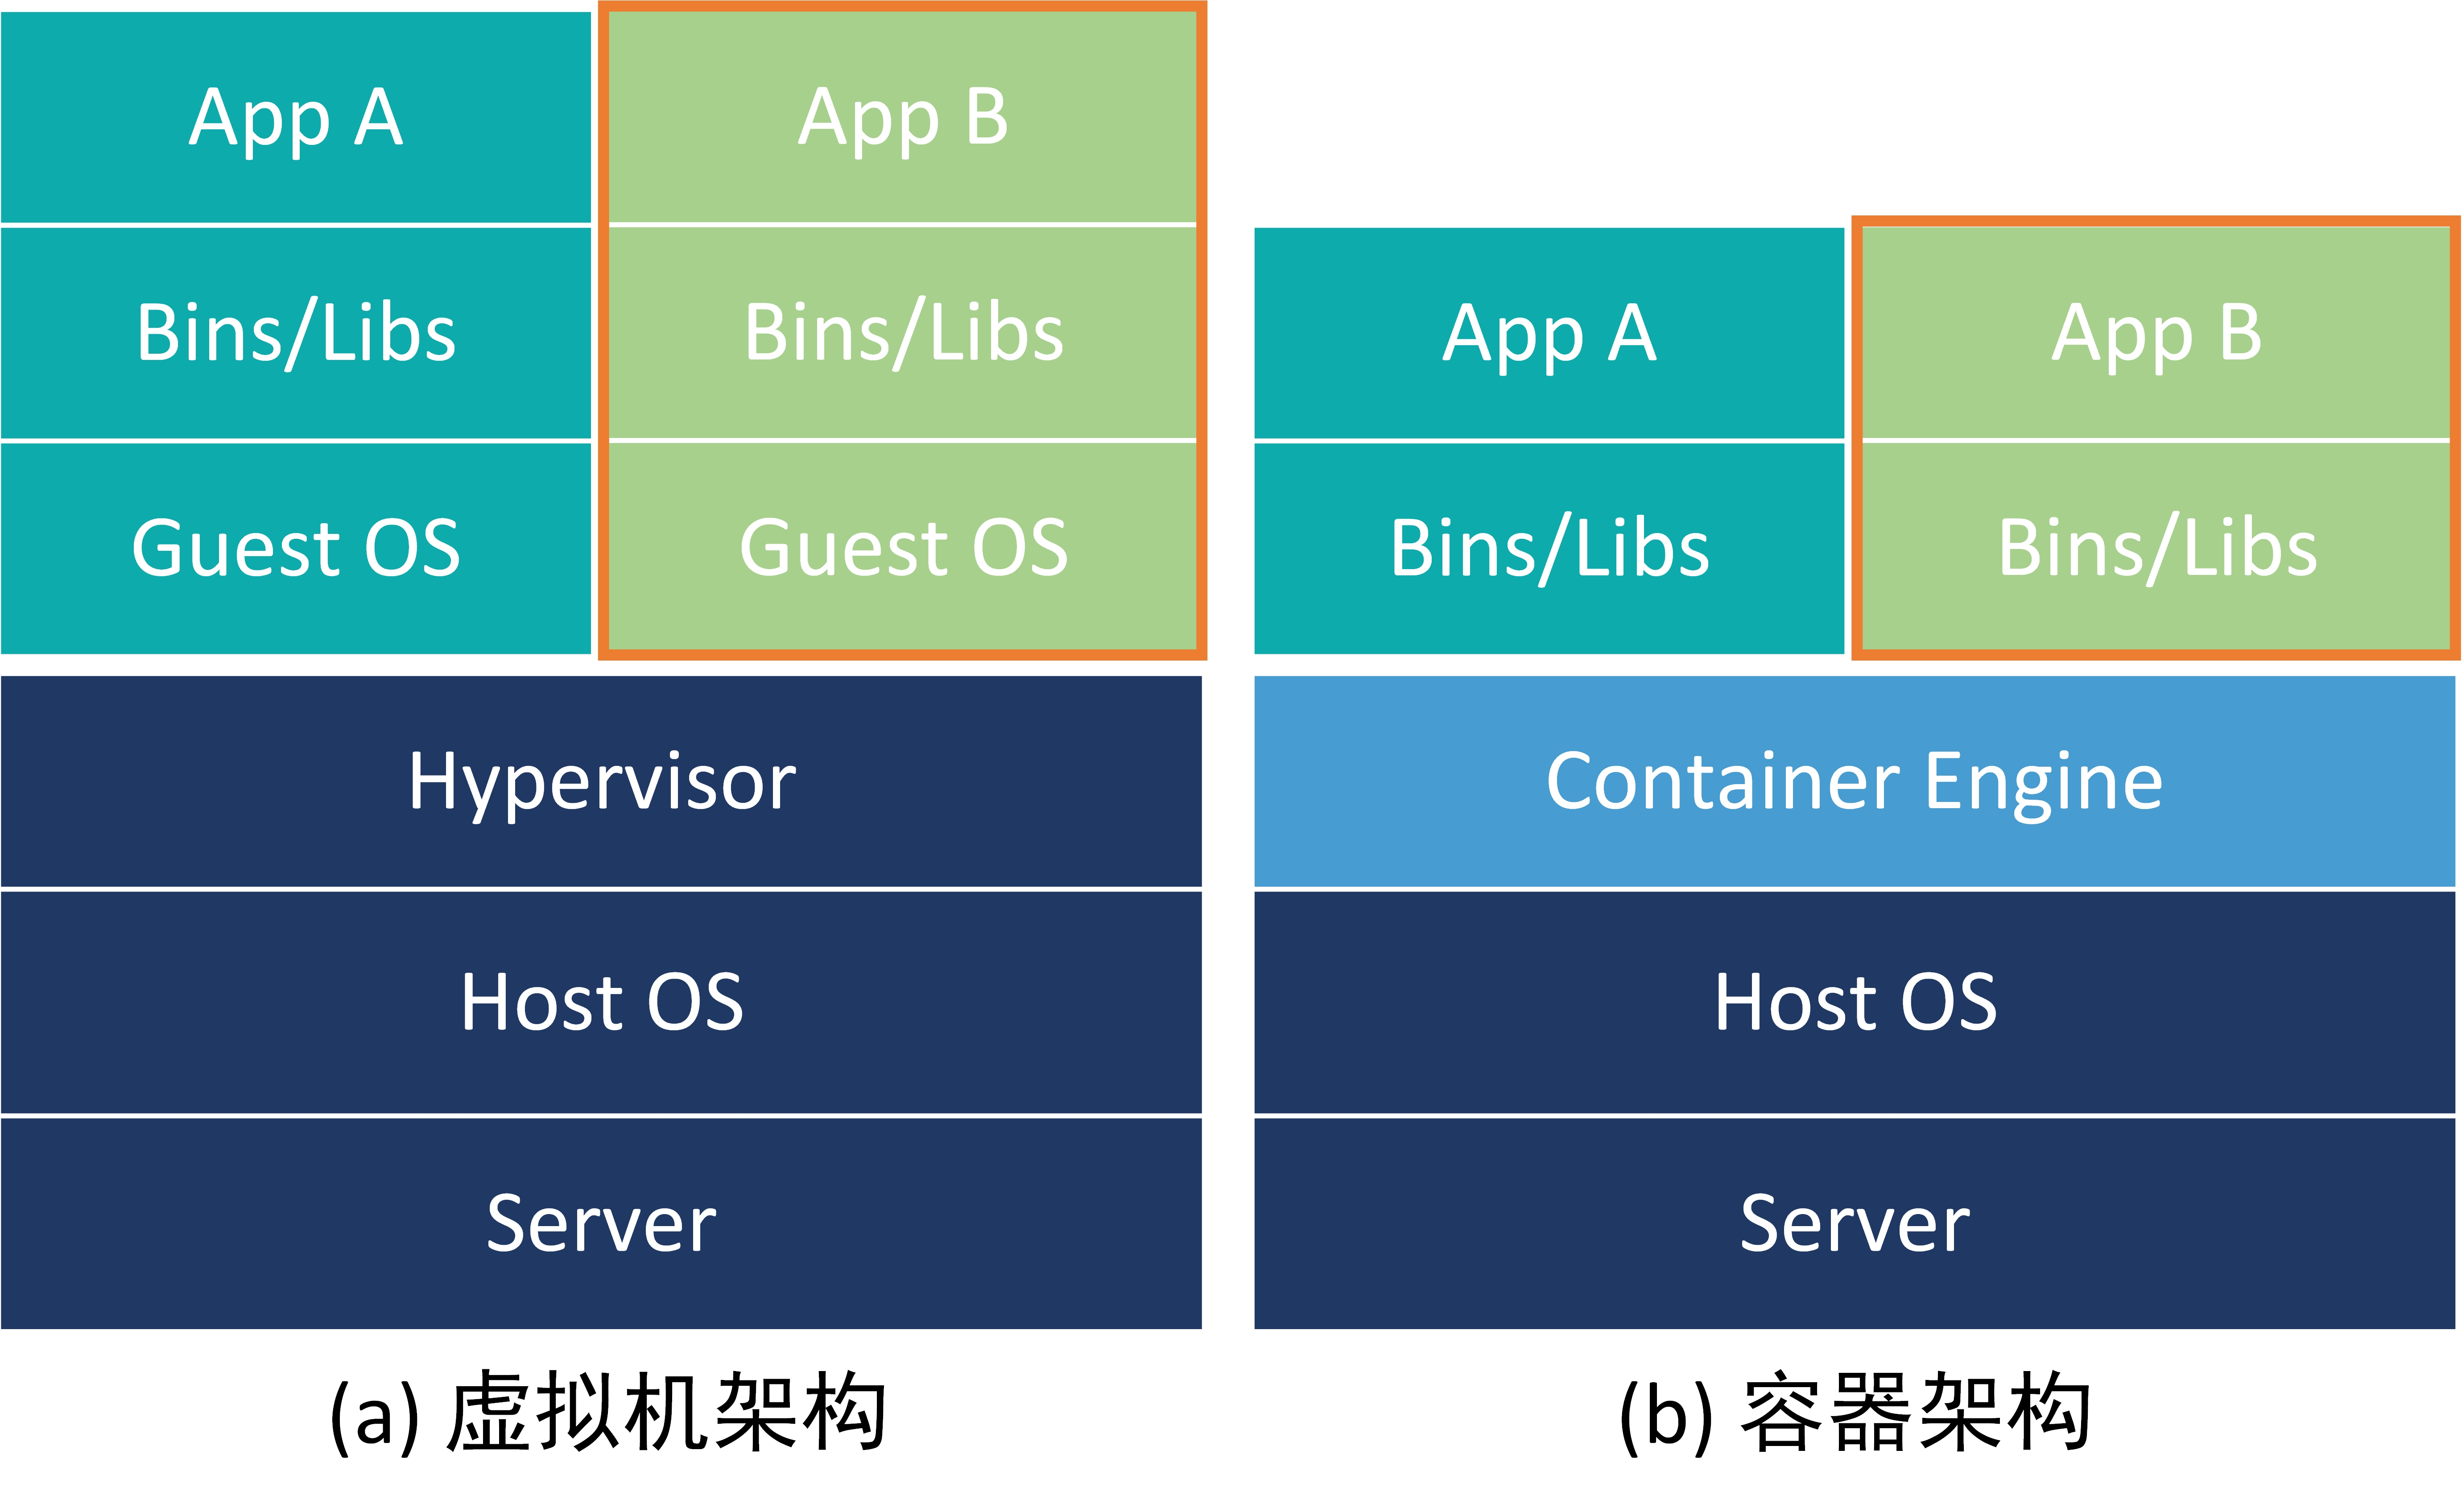
\includegraphics[scale=0.41]{figures/fig1_vm_vs_container.jpg}
    \caption{VM vs Container}
    \label{fig:fig1}
    \end{minipage}
}
\hspace{20pt}%
\visible<2->{
    \begin{minipage}{130pt}
    \centering
    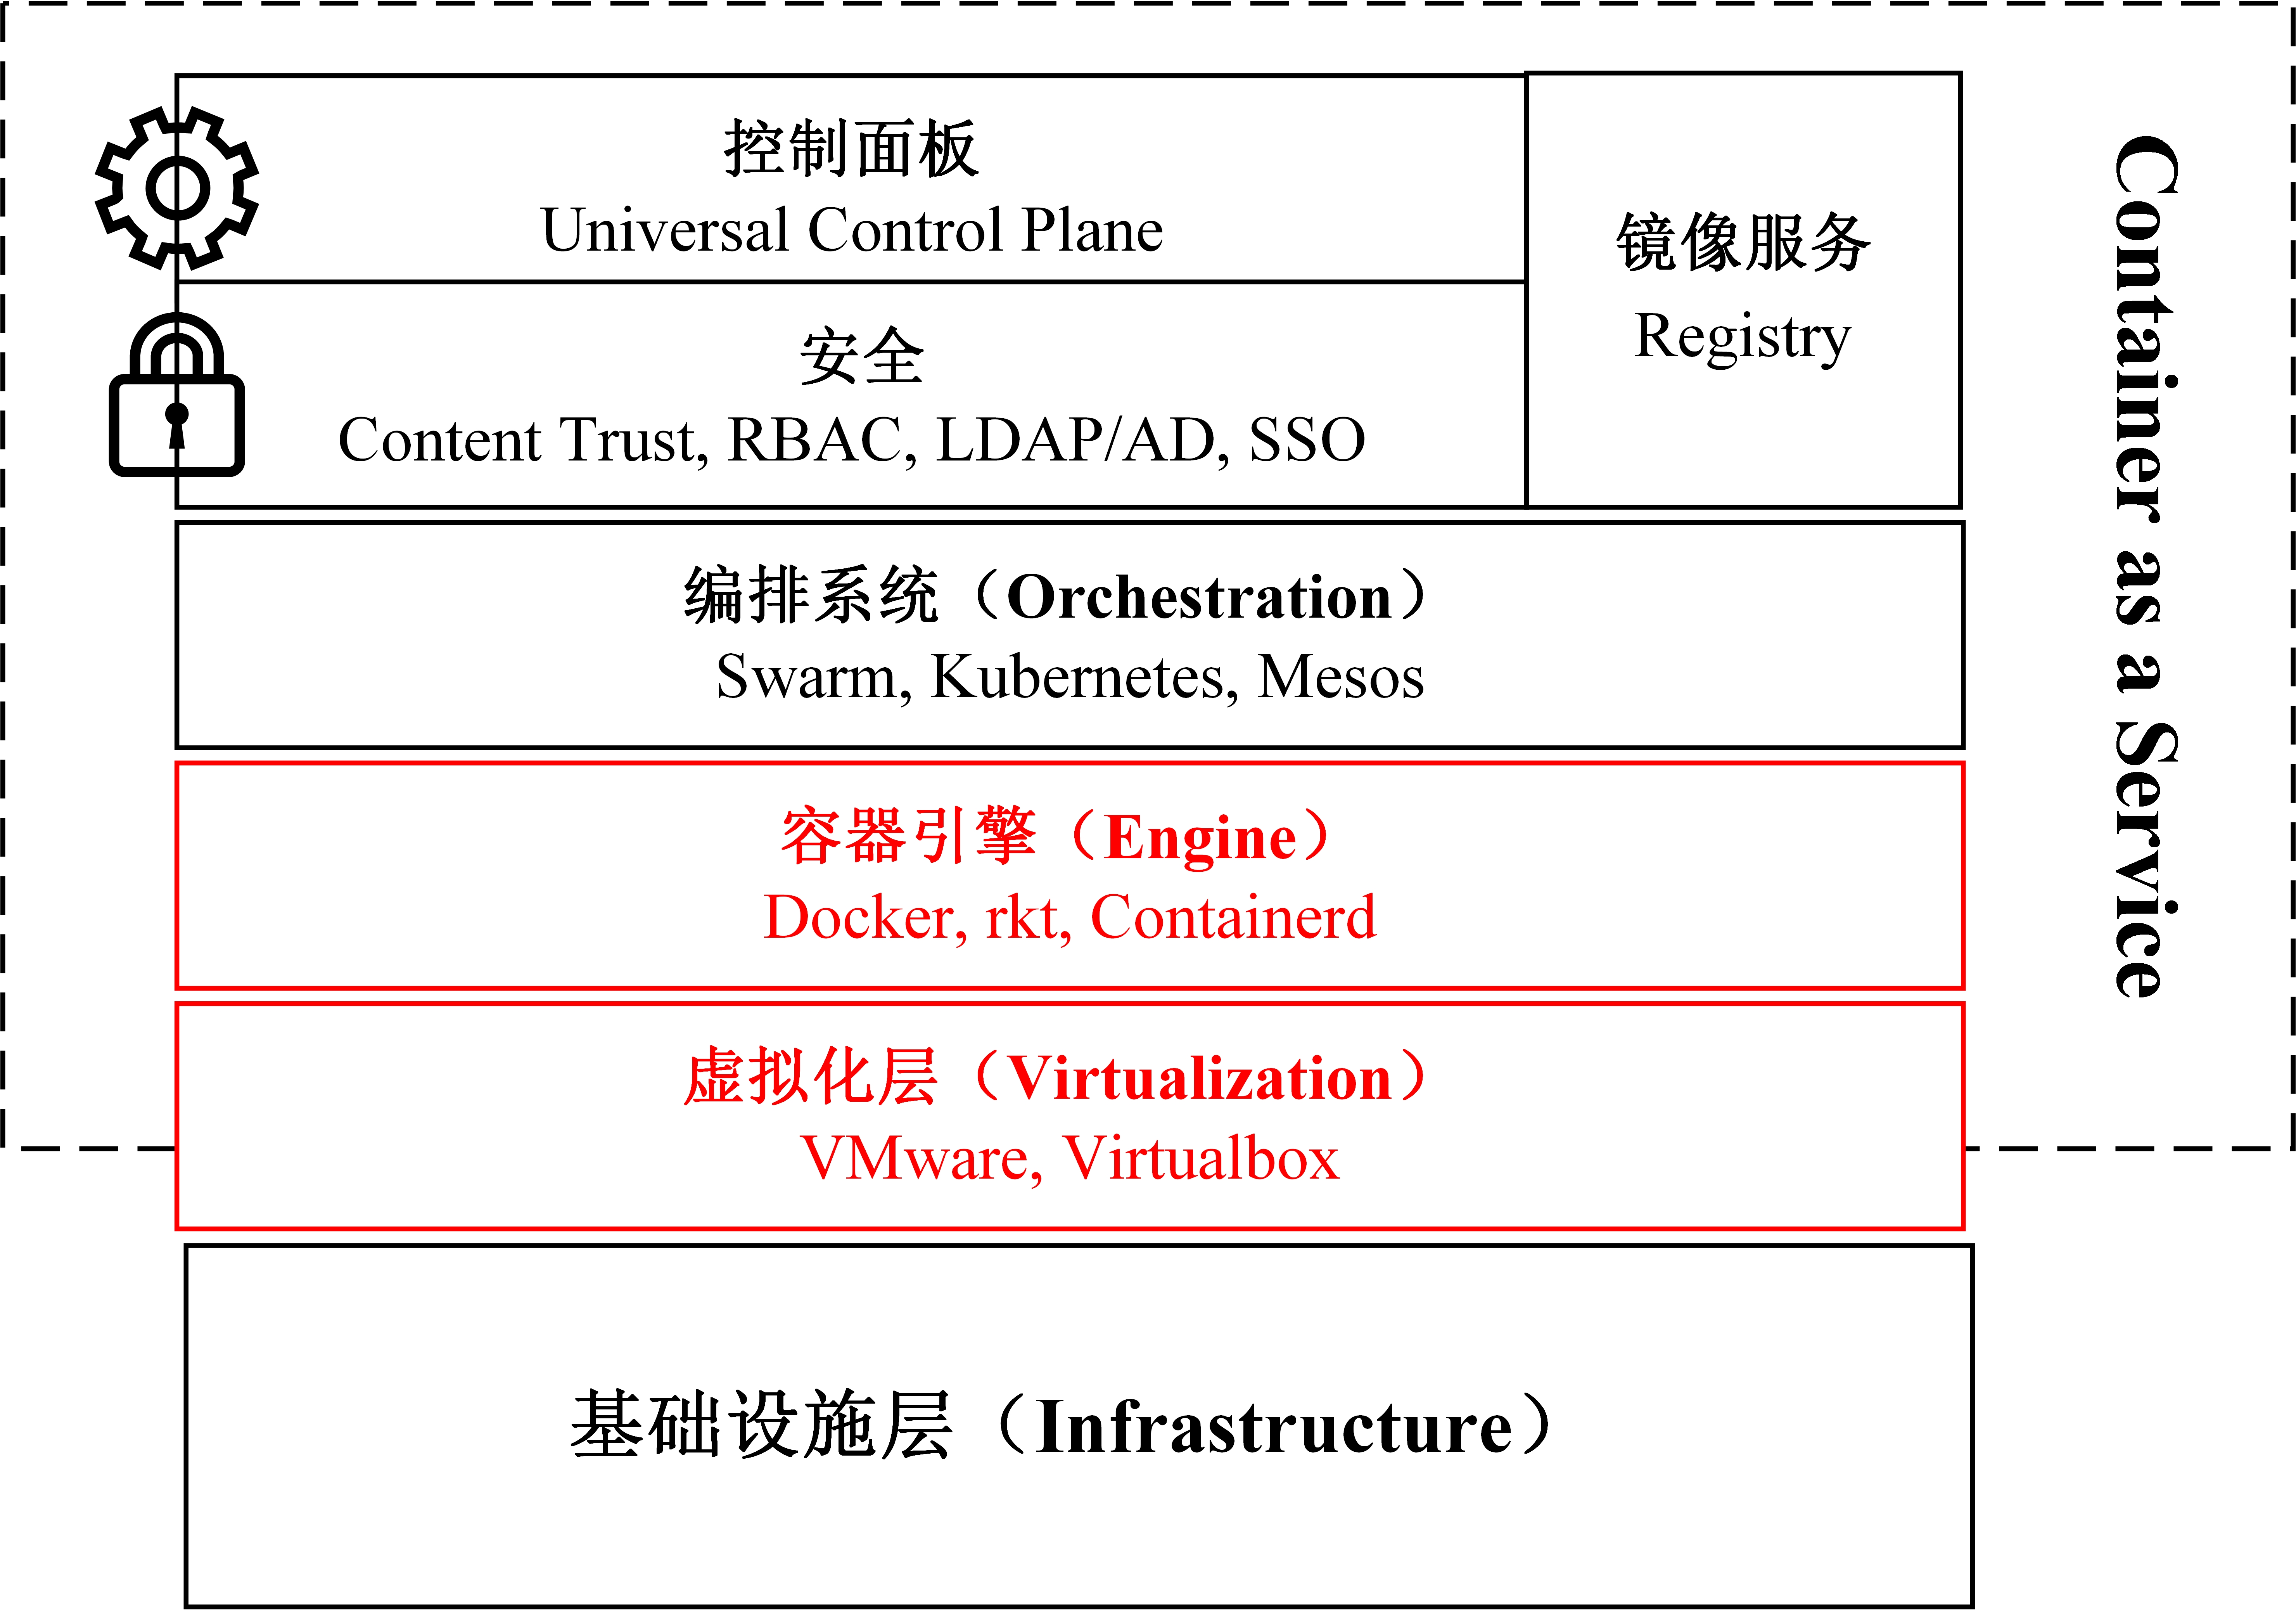
\includegraphics[scale=0.3]{figures/fig2_caas.jpg}
    \caption{CaaS架构示意图}
    \label{fig:fig2}
    \end{minipage}
}
\end{figure}

\end{frame}


%Motivation
%Title of section
\section{研究动机}

\subsection{主要目标}

\begin{frame}
\frametitle{研究动机}
\framesubtitle{主要目标}
\begin{block}{解决CaaS模式下云数据中心的能耗优化问题}
    \begin{itemize}
        \item 负载监控机制:负载与能耗紧密相关
        \begin{itemize}
            \item 实时性
            \item 准确性
            \item 易扩展性
        \end{itemize}
        \item 基于负载状态容器调度策略
        \begin{itemize}
            \item 保证云服务QoS(Quality of Service)
            \item 降低整体能耗
        \end{itemize}
    \end{itemize}
\end{block}
\end{frame}

\subsection{负载监控}

\begin{frame}
\frametitle{研究动机}
\framesubtitle{负载监控}
容器负载监控机制对云数据中心\textbf{\alert{资源配置和调度决策}}有较大影响

\begin{block}{负载监控机制}
\begin{itemize}
    \item<1-> 基于负载采集程序:负载变化频繁、异构网络环境导致滞后性
    \item<2-> 负载预测模型:主动进行资源配置和容器调度
\end{itemize}
\end{block}
\begin{figure}[htb]
\centering
    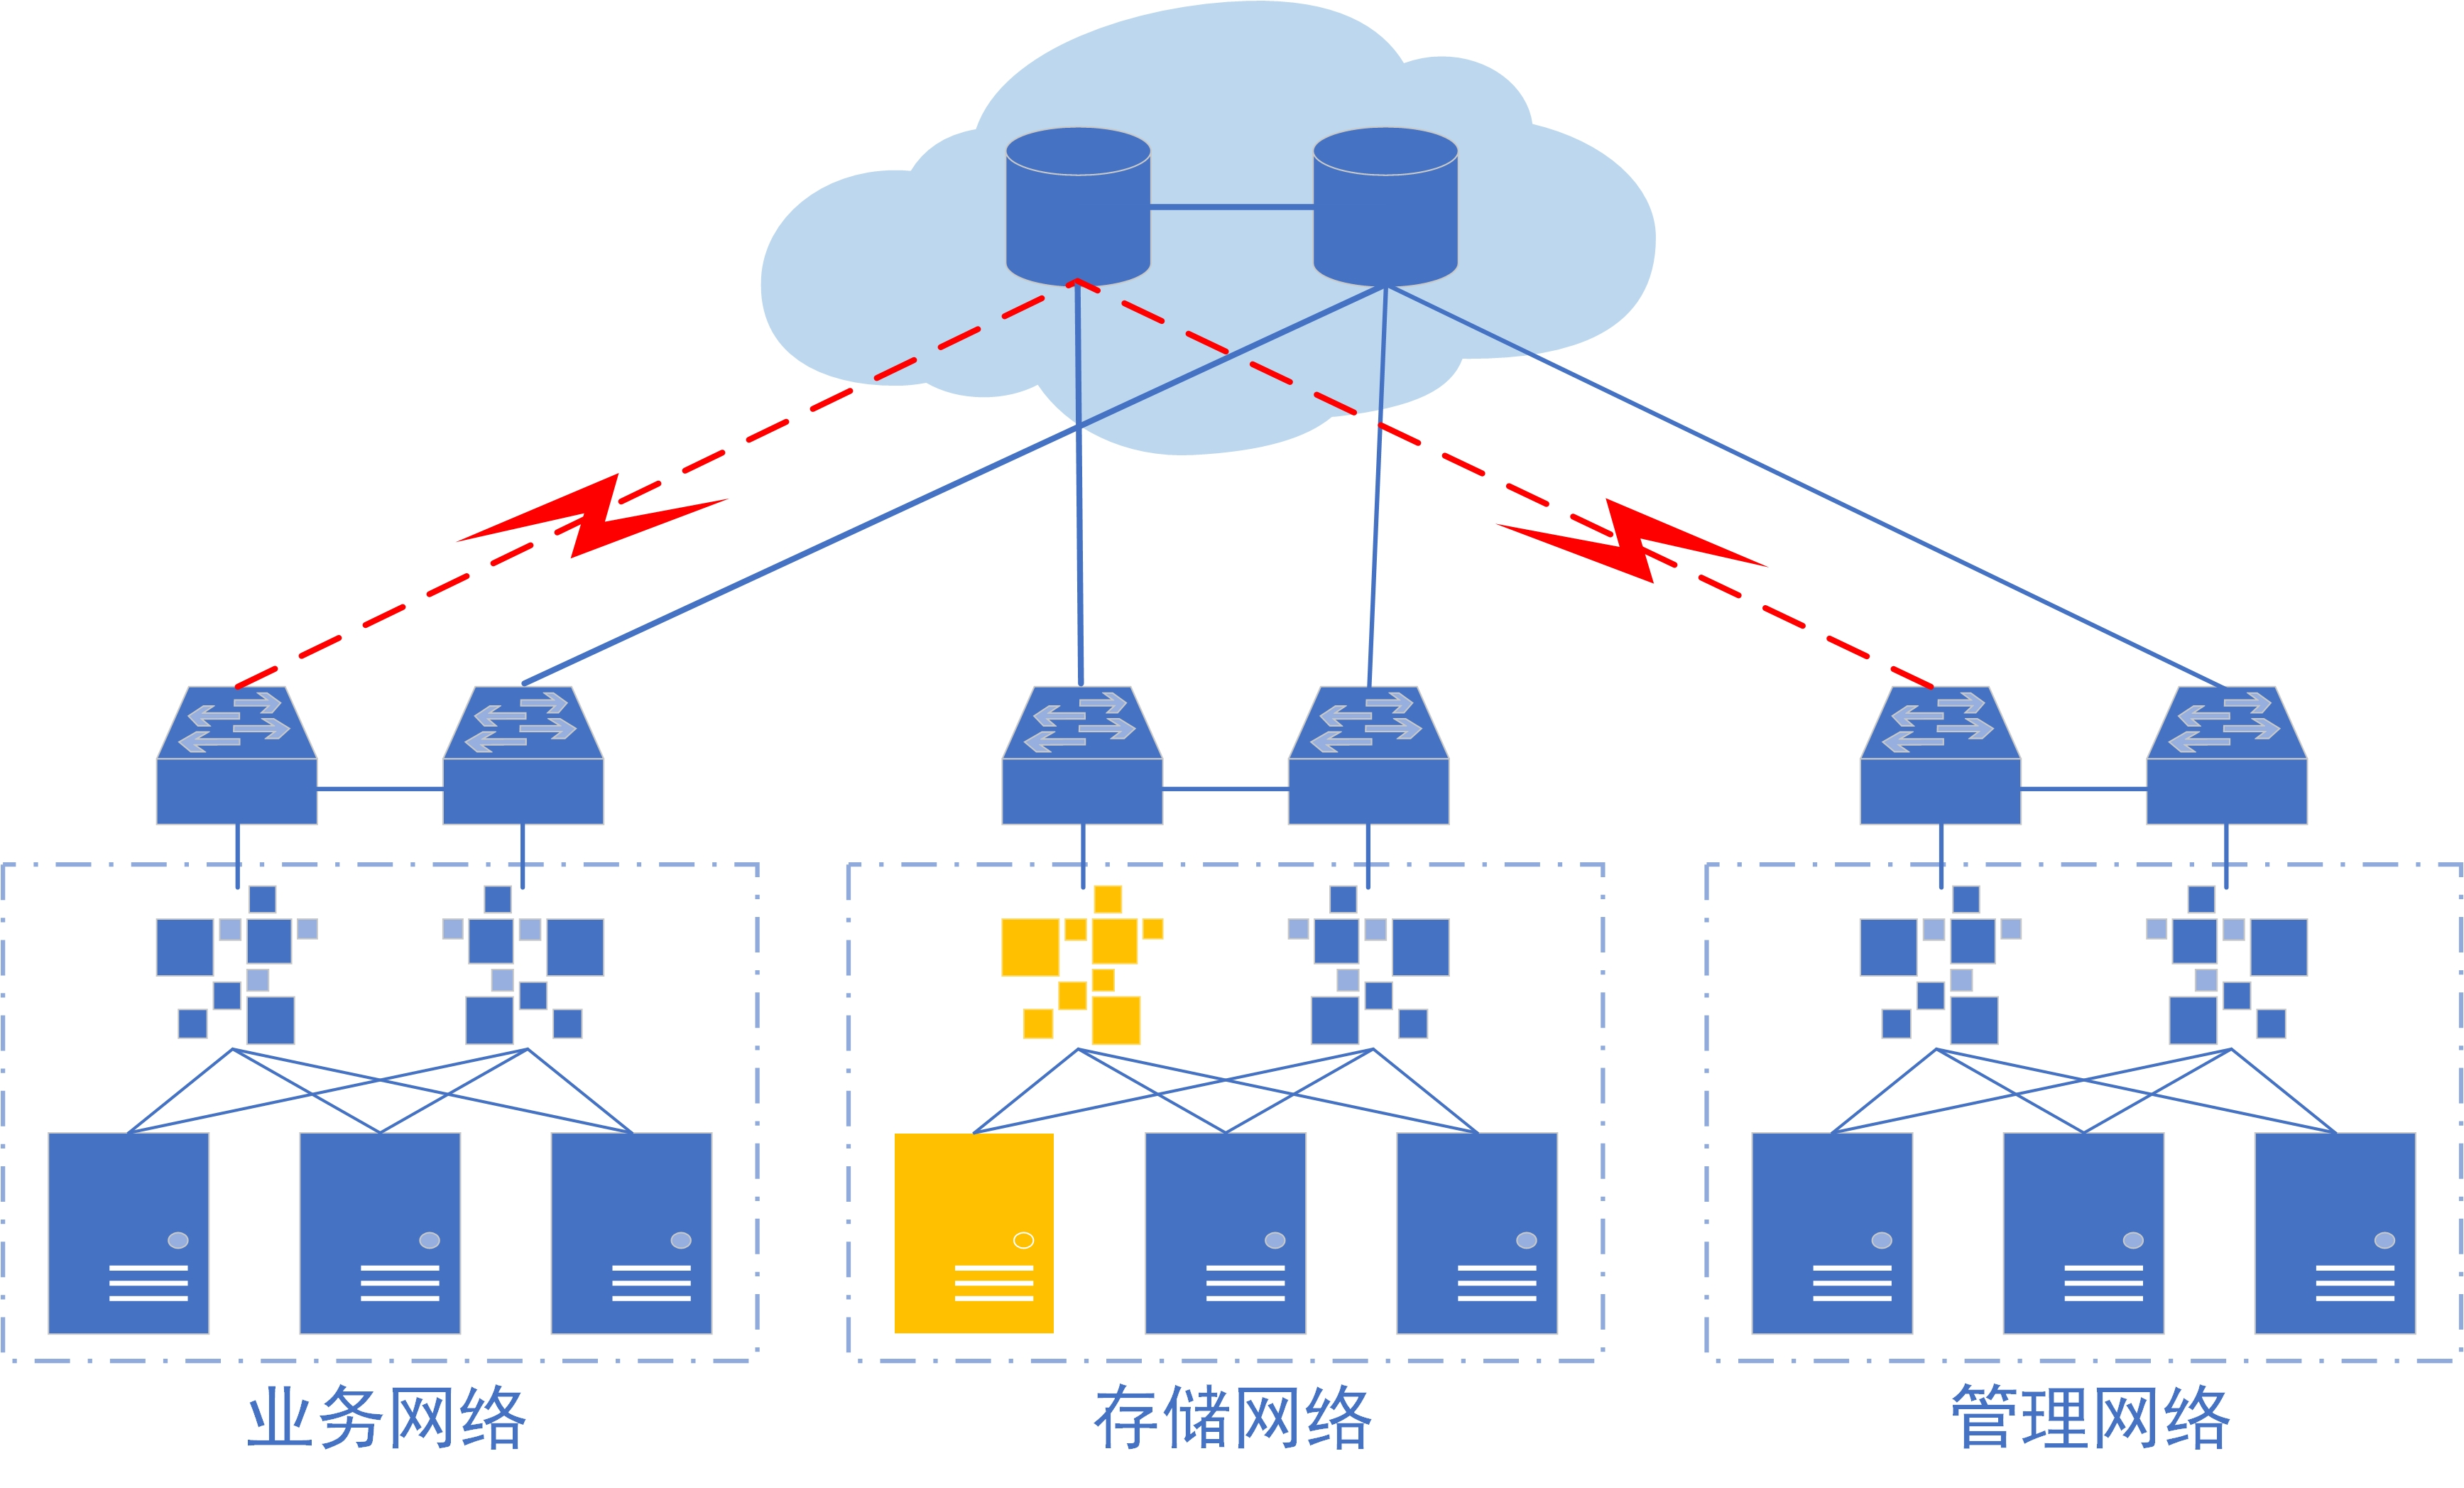
\includegraphics[scale=0.41]{figures/fig3_mmn.jpg}
    \caption{基于负载采集程序的监控网络}
    \label{fig:fig3}
\end{figure}
\end{frame}

\begin{frame}
\frametitle{研究动机}
\framesubtitle{负载监控}
\begin{block}{负载预测模型}
\begin{itemize}
    \item<1-1> 单值预测模型:预测特定值
    \begin{itemize}
        \item<1-1> \textbf{误差敏感} $\Rightarrow$ \textbf{决策失效}
        \item<1-1> \textbf{鲁棒性差} $\Rightarrow$ \textbf{决策过度}
    \end{itemize}
    \item<2-2> 区间预测模型:预测取值区间(置信度$\alpha=0.9$)
\end{itemize}
\end{block}

\vspace*{-0.7cm}
\visible<1>{
\begin{columns}
\begin{column}{0.6\textwidth}
    \centering
    \begin{table}[hftb]
    \centering
    \resizebox{\textwidth}{!}{%
        \begin{tabular}{ccl}
            \toprule
            \textbf{类型} & \textbf{模型名称} & \textbf{简述}\\
            \midrule
            \multirow{4}{*}{统计学模型} & ARIMA & 差分自回归移动平均\\
            ~ & Kalman滤波 & 基于递推演进和观测值对预测结果进行演进\\
            ~ & 排队论模型 & 基于在线作业请求和系统阻塞情况进行预测\\
            ~ & 灰色模型 & 模型新陈代谢过程,进行中长期预测\\
            \midrule
            \multirow{4}{*}{机器学习模型} & RNN & 递归神经网络预测\\
            ~ & BPNN & 原始信息前向传播,误差信息后向传播\\
            ~ & LSTM & 长短期记忆网络\\
            ~ & 混合模型 & 基于c-means聚类和模糊(Fuzzy)神经网络\\
            \bottomrule
        \end{tabular}
    }
    \caption{单值预测模型}
    \end{table}
\end{column}
\begin{column}{0.3\textwidth}
\centering
\begin{figure}[htb]
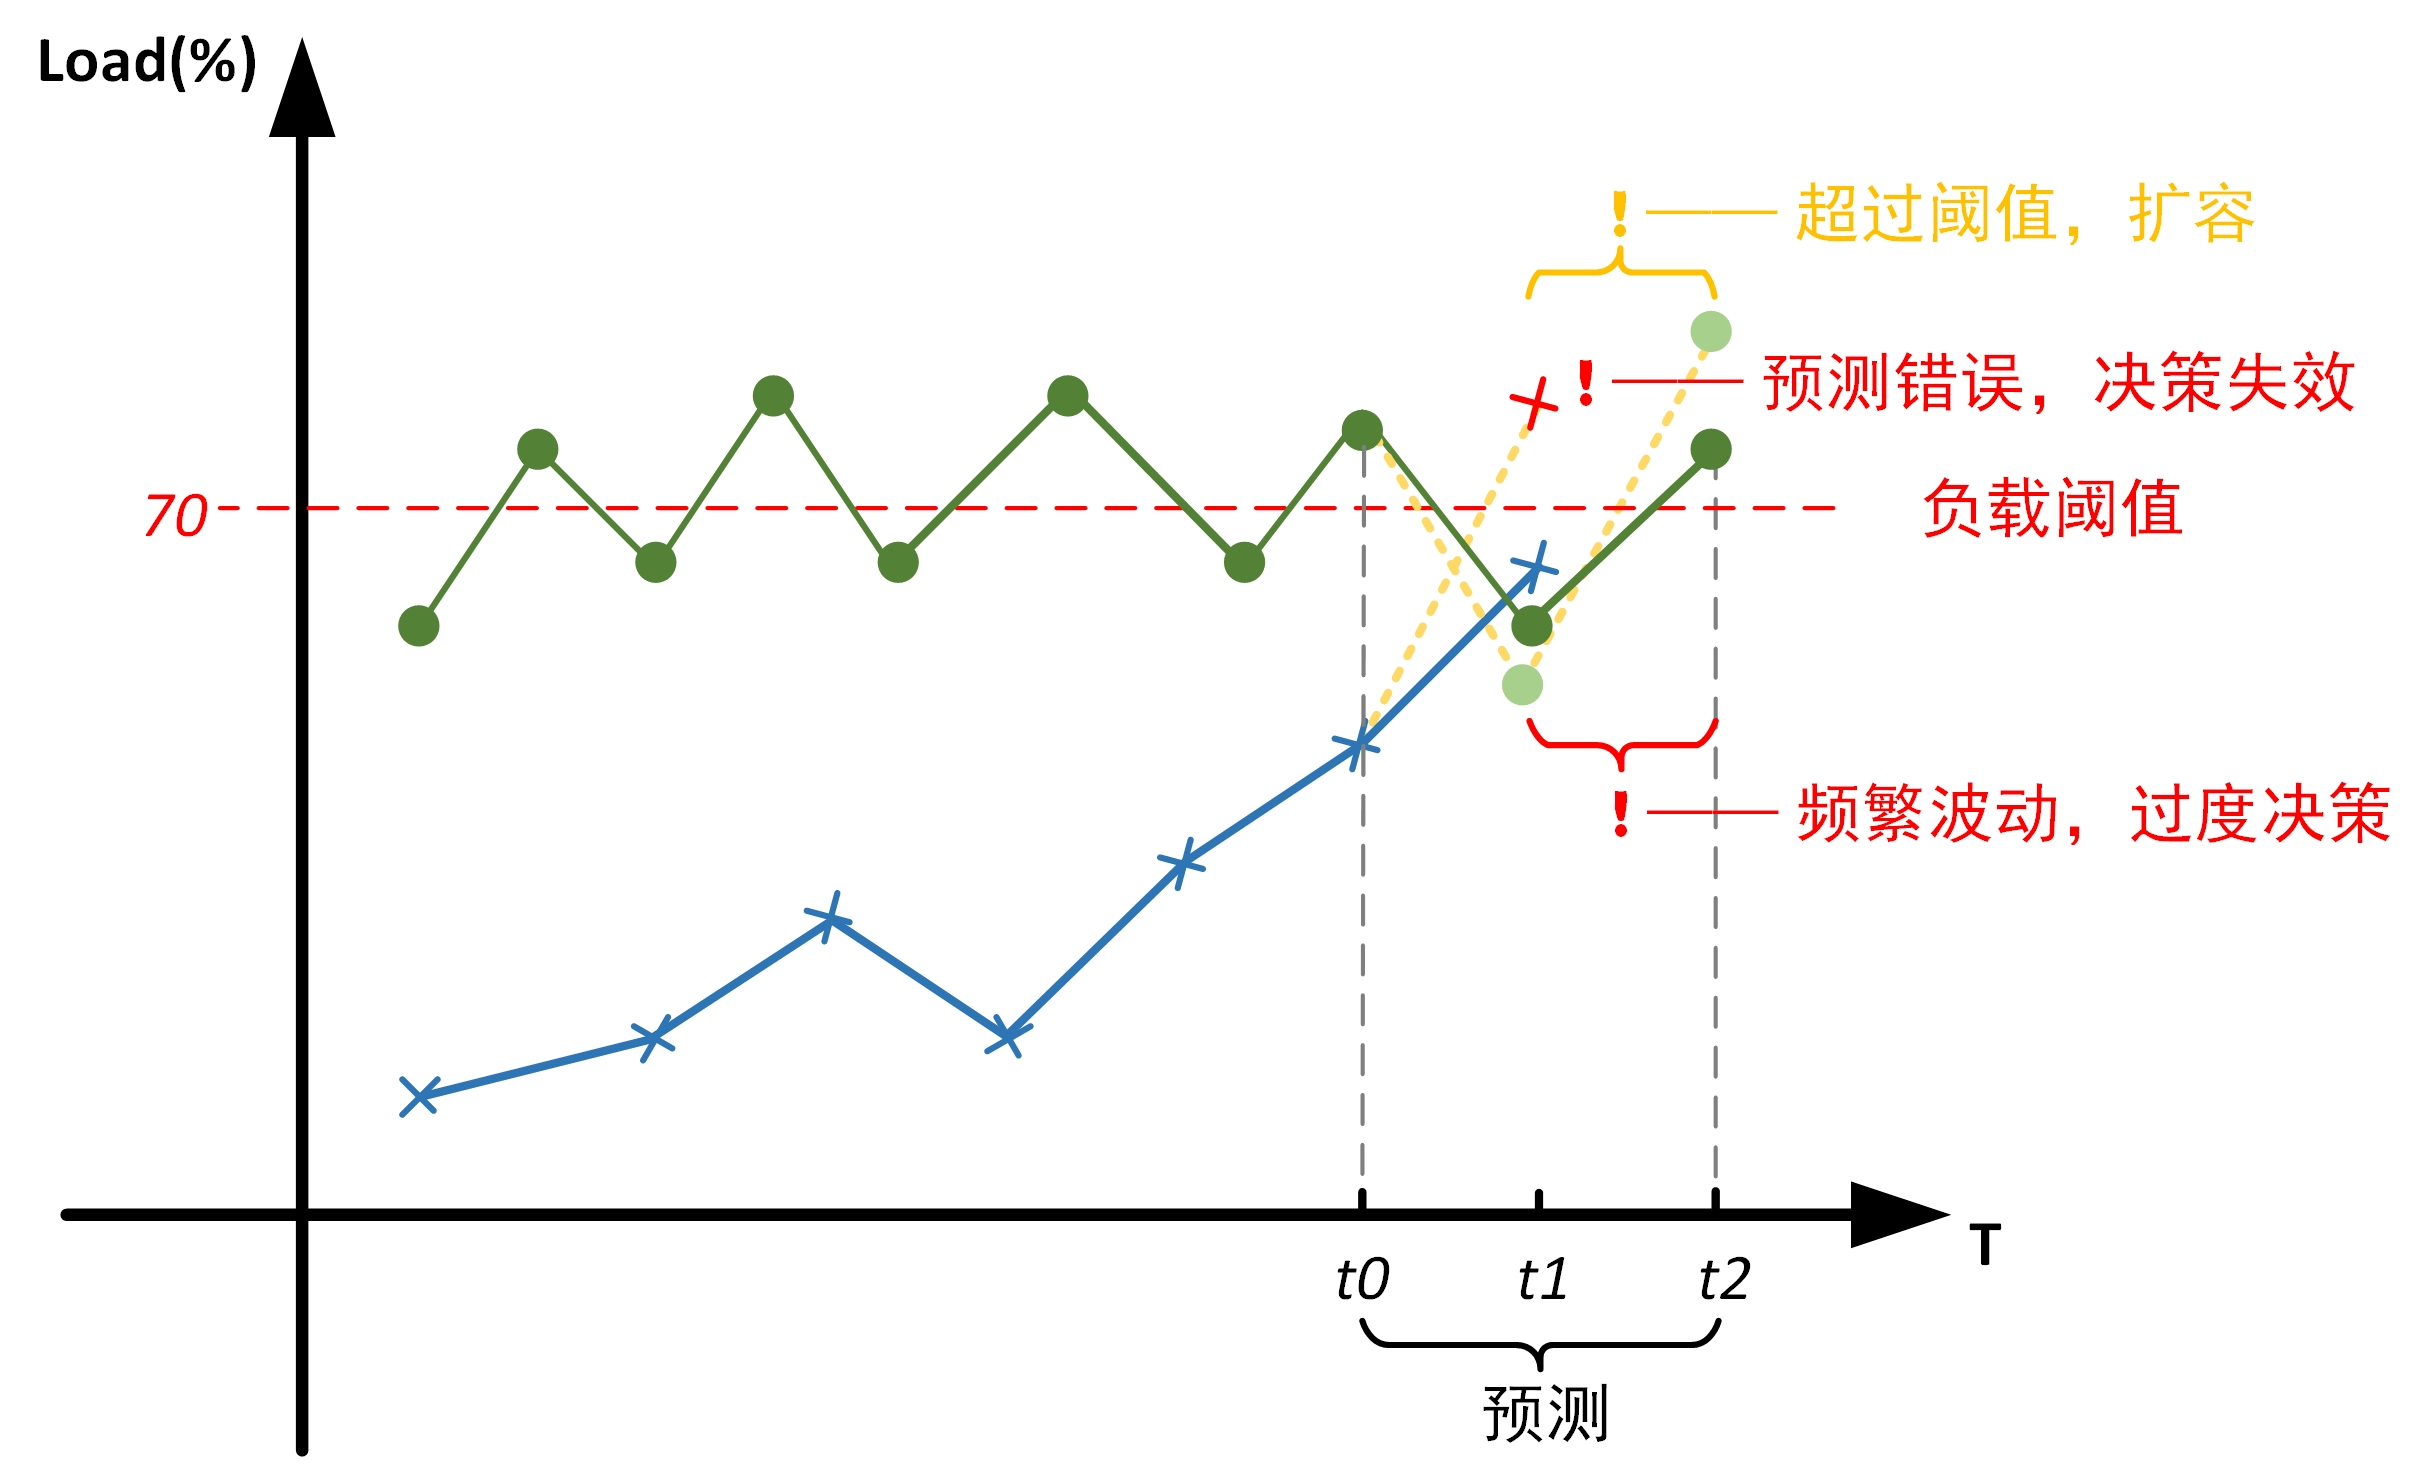
\includegraphics[scale=0.4]{figures/fig4_single_model.jpg}
\caption{单值预测模型}
\end{figure}
\end{column}
\end{columns}
}
\vspace*{-4.54cm}
\visible<2>{
\begin{columns}
\begin{column}{0.6\textwidth}
    \begin{table}[hftb]
    \centering
    \resizebox{\textwidth}{!}{%
        \begin{tabular}{ccl}
            \toprule
            \textbf{类型} & \textbf{模型名称} & \textbf{简述}\\
            \midrule
            概率论模型 & 贝叶斯模型 & 根据样本分布假设和统计学特征扩展区间\\
            \midrule
            \multirow{4}{*}{机器学习模型} & 线性回归 & \multirow{4}{*}{先拟合单值再根据分布假设构建区间}\\
            ~ & SVM & \\
            ~ & CART & \\
            ~ & 随机森林 & \\
            \bottomrule
        \end{tabular}
    }
    \caption{区间预测模型}
    \end{table}
\end{column}
\begin{column}{0.3\textwidth}
\end{column}
\end{columns}
}
\end{frame}

\subsection{容器调度}

\begin{frame}
\frametitle{研究动机}
\framesubtitle{容器调度}
\end{frame}

%Model
%Title of section
\section{容器负载预测模型}

\subsection{模型结构}

\begin{frame}
\frametitle{模型结构}
\framesubtitle{引言}
\begin{itemize}
    \item 单值预测模型:ARIMA、Kalman滤波、神经网络、……
    \begin{itemize}
        \item \textbf{误差敏感} $\Rightarrow$ \textbf{决策失效}
        \item \textbf{鲁棒性差} $\Rightarrow$ \textbf{决策过度}
    \end{itemize}
    \item 区间预测模型:贝叶斯、回归模型、随机森林、……
    \begin{itemize}
        \item \textbf{预测区间} $\Rightarrow$ \textbf{目标不确定性(包含误差)}
        \item \textbf{区间置信度} $\Rightarrow$ \textbf{适合决策}
        \item \alert{\textbf{先预测再扩展为区间} $\Rightarrow$ \textbf{先验假设}}
        \item \alert{\textbf{相同分布假设} $\nRightarrow$ \textbf{适应不同类型负载}}
    \end{itemize}
    \item 基于趋势感知的区间预测模型:SAC-GPSO-SVM
    \begin{itemize}
        \item \textbf{趋势感知} $\Rightarrow$ \textbf{平稳型、趋势型和周期型负载}
        \item \textbf{区间构造} $\Rightarrow$ \textbf{针对不同负载类型}
        \item \textbf{区间预测} $\Rightarrow$ \textbf{先构建区间再预测}(\sout{先预测再扩展为区间})
        \item \textbf{实时预测} $\Rightarrow$ \textbf{预测效率}(模型训练和预测结果计算)
    \end{itemize}
\end{itemize}
\end{frame}

\begin{frame}
\frametitle{模型结构}
\framesubtitle{示意图}
\begin{columns}
\begin{column}{0.4\textwidth}
\begin{figure}[htb]
\centering

\includegraphics[scale=0.3]{figures/fig6_sac-gpso-svm.jpg}
\caption{基于趋势感知的区间预测模型}
\label{fig:fig6}
\end{figure}
\end{column}
\begin{column}{0.6\textwidth}
\begin{figure}[htb]
\centering
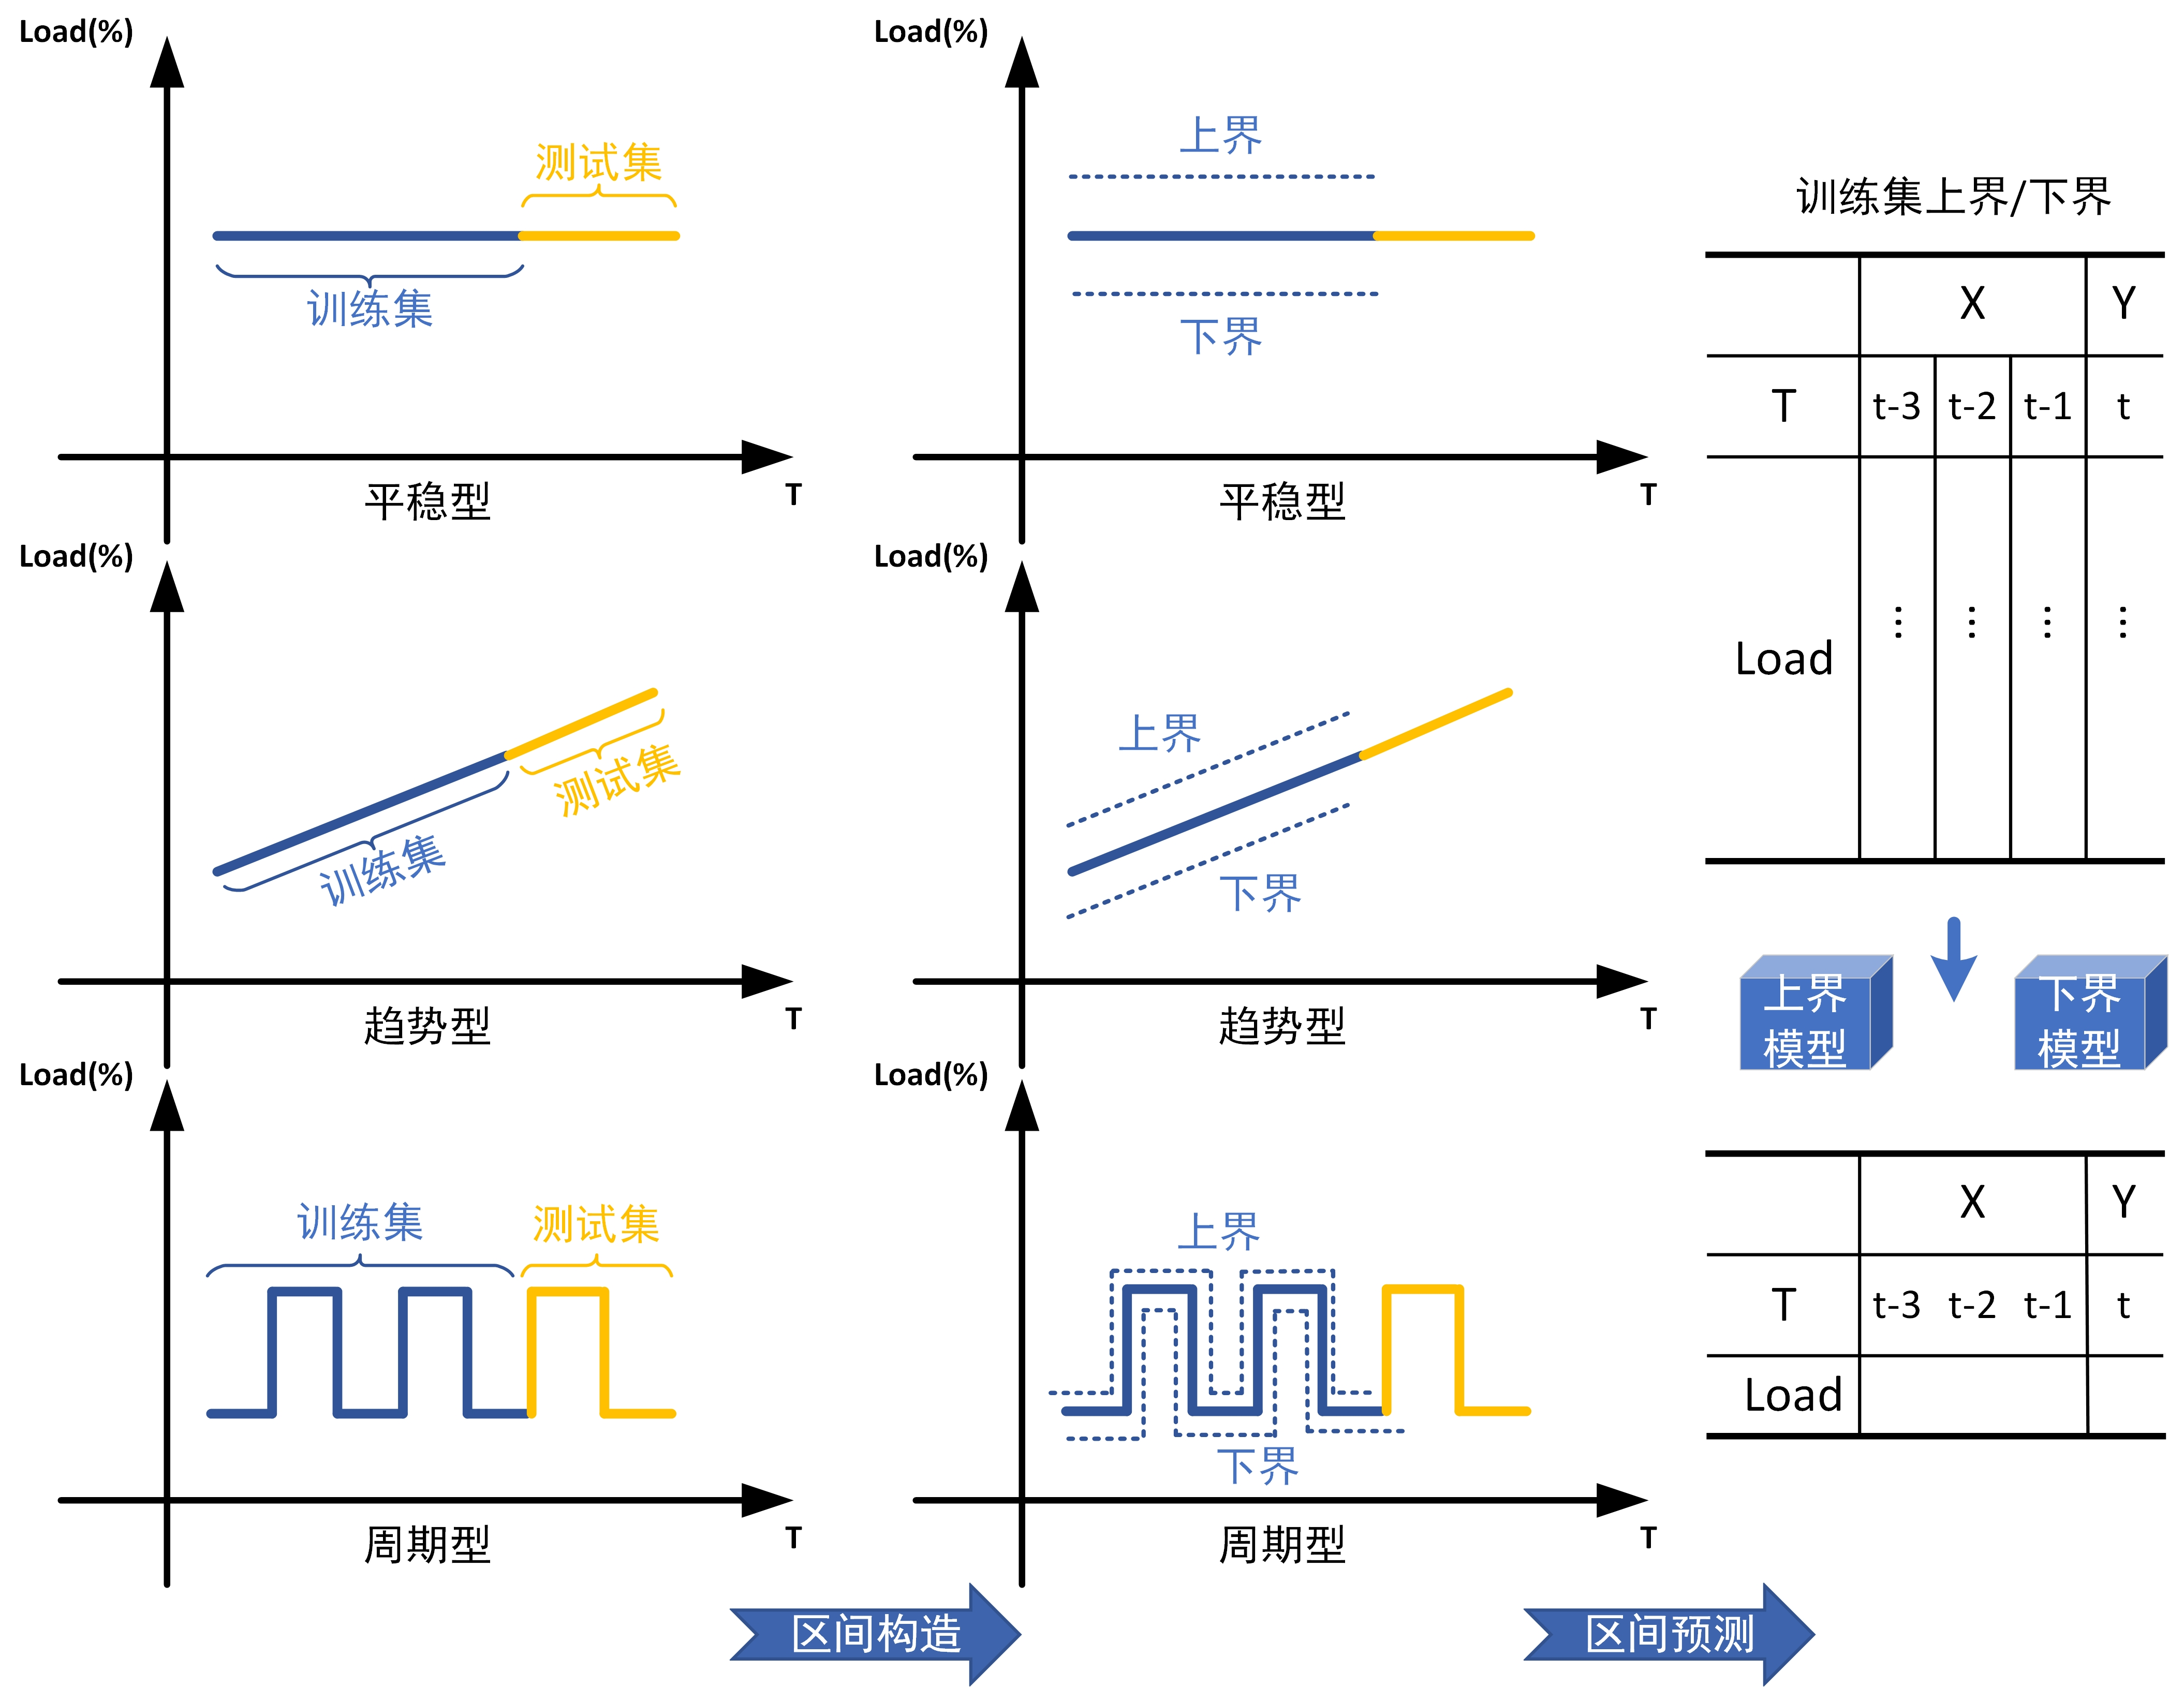
\includegraphics[scale=0.38]{figures/fig7_predict_process.jpg}
\caption{模型预测过程}
\label{fig:fig6}
\end{figure}
\end{column}
\end{columns}
\end{frame}

\subsection{趋势感知}

\begin{frame}
\frametitle{趋势感知}
\framesubtitle{定义}
\end{frame}

\begin{frame}
\frametitle{趋势感知}
\framesubtitle{频谱特征分析}
\end{frame}

\begin{frame}
\frametitle{趋势感知}
\framesubtitle{自相关系数分析}
\end{frame}

\subsection{区间构造}

\begin{frame}
\frametitle{区间构造}
\end{frame}


\subsection{区间预测}

\begin{frame}
\frametitle{区间预测}
\end{frame}


\subsection{实验结果与分析}

\begin{frame}
\frametitle{实验结果与分析}
\end{frame}

%Scheduler
%Title of section
\section{基于动态伸缩的容器调度策略}

\subsection{问题定义}

\begin{frame}
\frametitle{问题定义}
\framesubtitle{调度目标}
\begin{itemize}
    \item 最小化CaaS数据中心总能耗
    \begin{equation}
    \begin{align*}
            &\min\quad P_{dc}(t)=\sum_{i=1}^{N_s} P_i(t) \\
            &s.t.\quad
            \begin{cases}
            \sum_{j=1}^{N_{vm}}vm_{(j,i,r)}(t) < S_(i,r),\\
            \forall i \in [1,N_s],\ \forall r \in \{CPU,Memory,Disk,BW\} \\
            \\
            \sum_{k=1}^{N_{c}}c_{(k,j,i,r)}(t) < vm_(j,i,r),\\
            \forall i \in [1,N_{vm}],\ \forall r \in \{CPU,Memory,Disk,BW\}
            \end{cases}
    \end{align*}
    \end{equation}
\end{itemize}
\end{frame}

\subsection{系统结构}

\begin{frame}
\frametitle{系统结构}
\framesubtitle{调度系统模型}
\begin{exampleblock}{调度系统模型设计思路}
\begin{itemize}
    \item 主机状态模块:标记高负载/低负载主机
    \begin{itemize}
            \item 高负载主机列表
            \item 低负载主机列表
    \end{itemize}
    \item 容器状态模块
    \begin{itemize}
        \item 负载预测结果与调整阈值 $\Rightarrow$ 计算容器扩容、缩容数量
        \item 从高负载主机列表中选择需要迁移容器
    \end{itemize}
    \item 容器调度模块
     \begin{itemize}
             \item 为待迁移容器找到目的地
             \item 基于资源约束条件合并低负载主机上的容器
             \item 销毁并关闭空载的虚拟机和服务器 $\Rightarrow$ 避免不必要的能耗
     \end{itemize}
\end{itemize}
\end{exampleblock}
\end{frame}

\begin{frame}
\frametitle{系统结构}
\framesubtitle{调度系统示意图}
\begin{figure}[htb]
    \centering
    \includegraphics[width=0.5\textwidth]{figures/fig14_scheduler_sys.jpg}
    \caption{基于动态伸缩的容器调度系统结构}
    \label{fig:fig14}
\end{figure}
\bigskip
\end{frame}

\subsection{调度算法}

\begin{frame}
\frametitle{调度算法}
\framesubtitle{主机状态模块(1/1):主机状态标记算法 - 标记主机状态}
\begin{itemize}
    \item 主机状态标记:通过\textbf{静态阈值法}设置$T_{ol}$和$T_{ul}$
    \begin{equation}
        Host\ status =
        \begin{cases}
            \textbf{Over-Load} \ \ \ if \ U_i(t) > T_{ol} \\
            \textbf{Under-Load} \ \ if\ U_i(t) < T_{ul}
        \end{cases}
    \end{equation}
\end{itemize}
\end{frame}

\begin{frame}
\frametitle{调度算法}
\framesubtitle{容器状态模块(1/2):容器伸缩算法 - 计算容器扩缩容数量}
\begin{itemize}
    \item 令应用$V$的当前容器副本总数$n=n_{now}$
    \begin{itemize}
        \item 应用$V$负载上界:$L_v^u = \sum_{i=1}^{n_{now}}l_i^u$
        \item 应用$V$负载下界:$L_v^l = \sum_{i=1}^{n_{now}}l_i^l$
    \end{itemize}
    \item 设置用于应用$V$扩缩容的调整阈值为$L_v$
        \begin{itemize}
            \item 满足公式\ref{eq:lu}(负载落在$L_v$之上) $\Rightarrow$ 扩容 $\lceil \frac{(L_v^u+L_v^l)}{2L_v} - n_{now} \rceil$ 个
            \item 满足公式\ref{eq:ll}(负载落在$L_v$之下)  $\Rightarrow$ 缩容$\lceil n_{now} - \frac{(L_v^u+L_v^l)}{2L_v} {\color{red} - 1}\rceil$ 个
        \end{itemize}
    \begin{equation}
        \frac{L_v^u - n_{now} \times L_v}{n_{now} \times L_v - L^l_v} > 1
        \label{eq:lu}
    \end{equation}
    \begin{equation}
        \frac{(n_{now} - 1) \times L_v - L_v^l}{L_v^u - (n_{now} - 1) \times L_v} > 1
        \label{eq:ll}
    \end{equation}
\end{itemize}
\end{frame}

\begin{frame}
\frametitle{调度算法}
\framesubtitle{容器状态模块(2/2):容器选择算法 - 选择高负载主机上需要迁移容器}
\begin{figure}[htb]
    \centering
    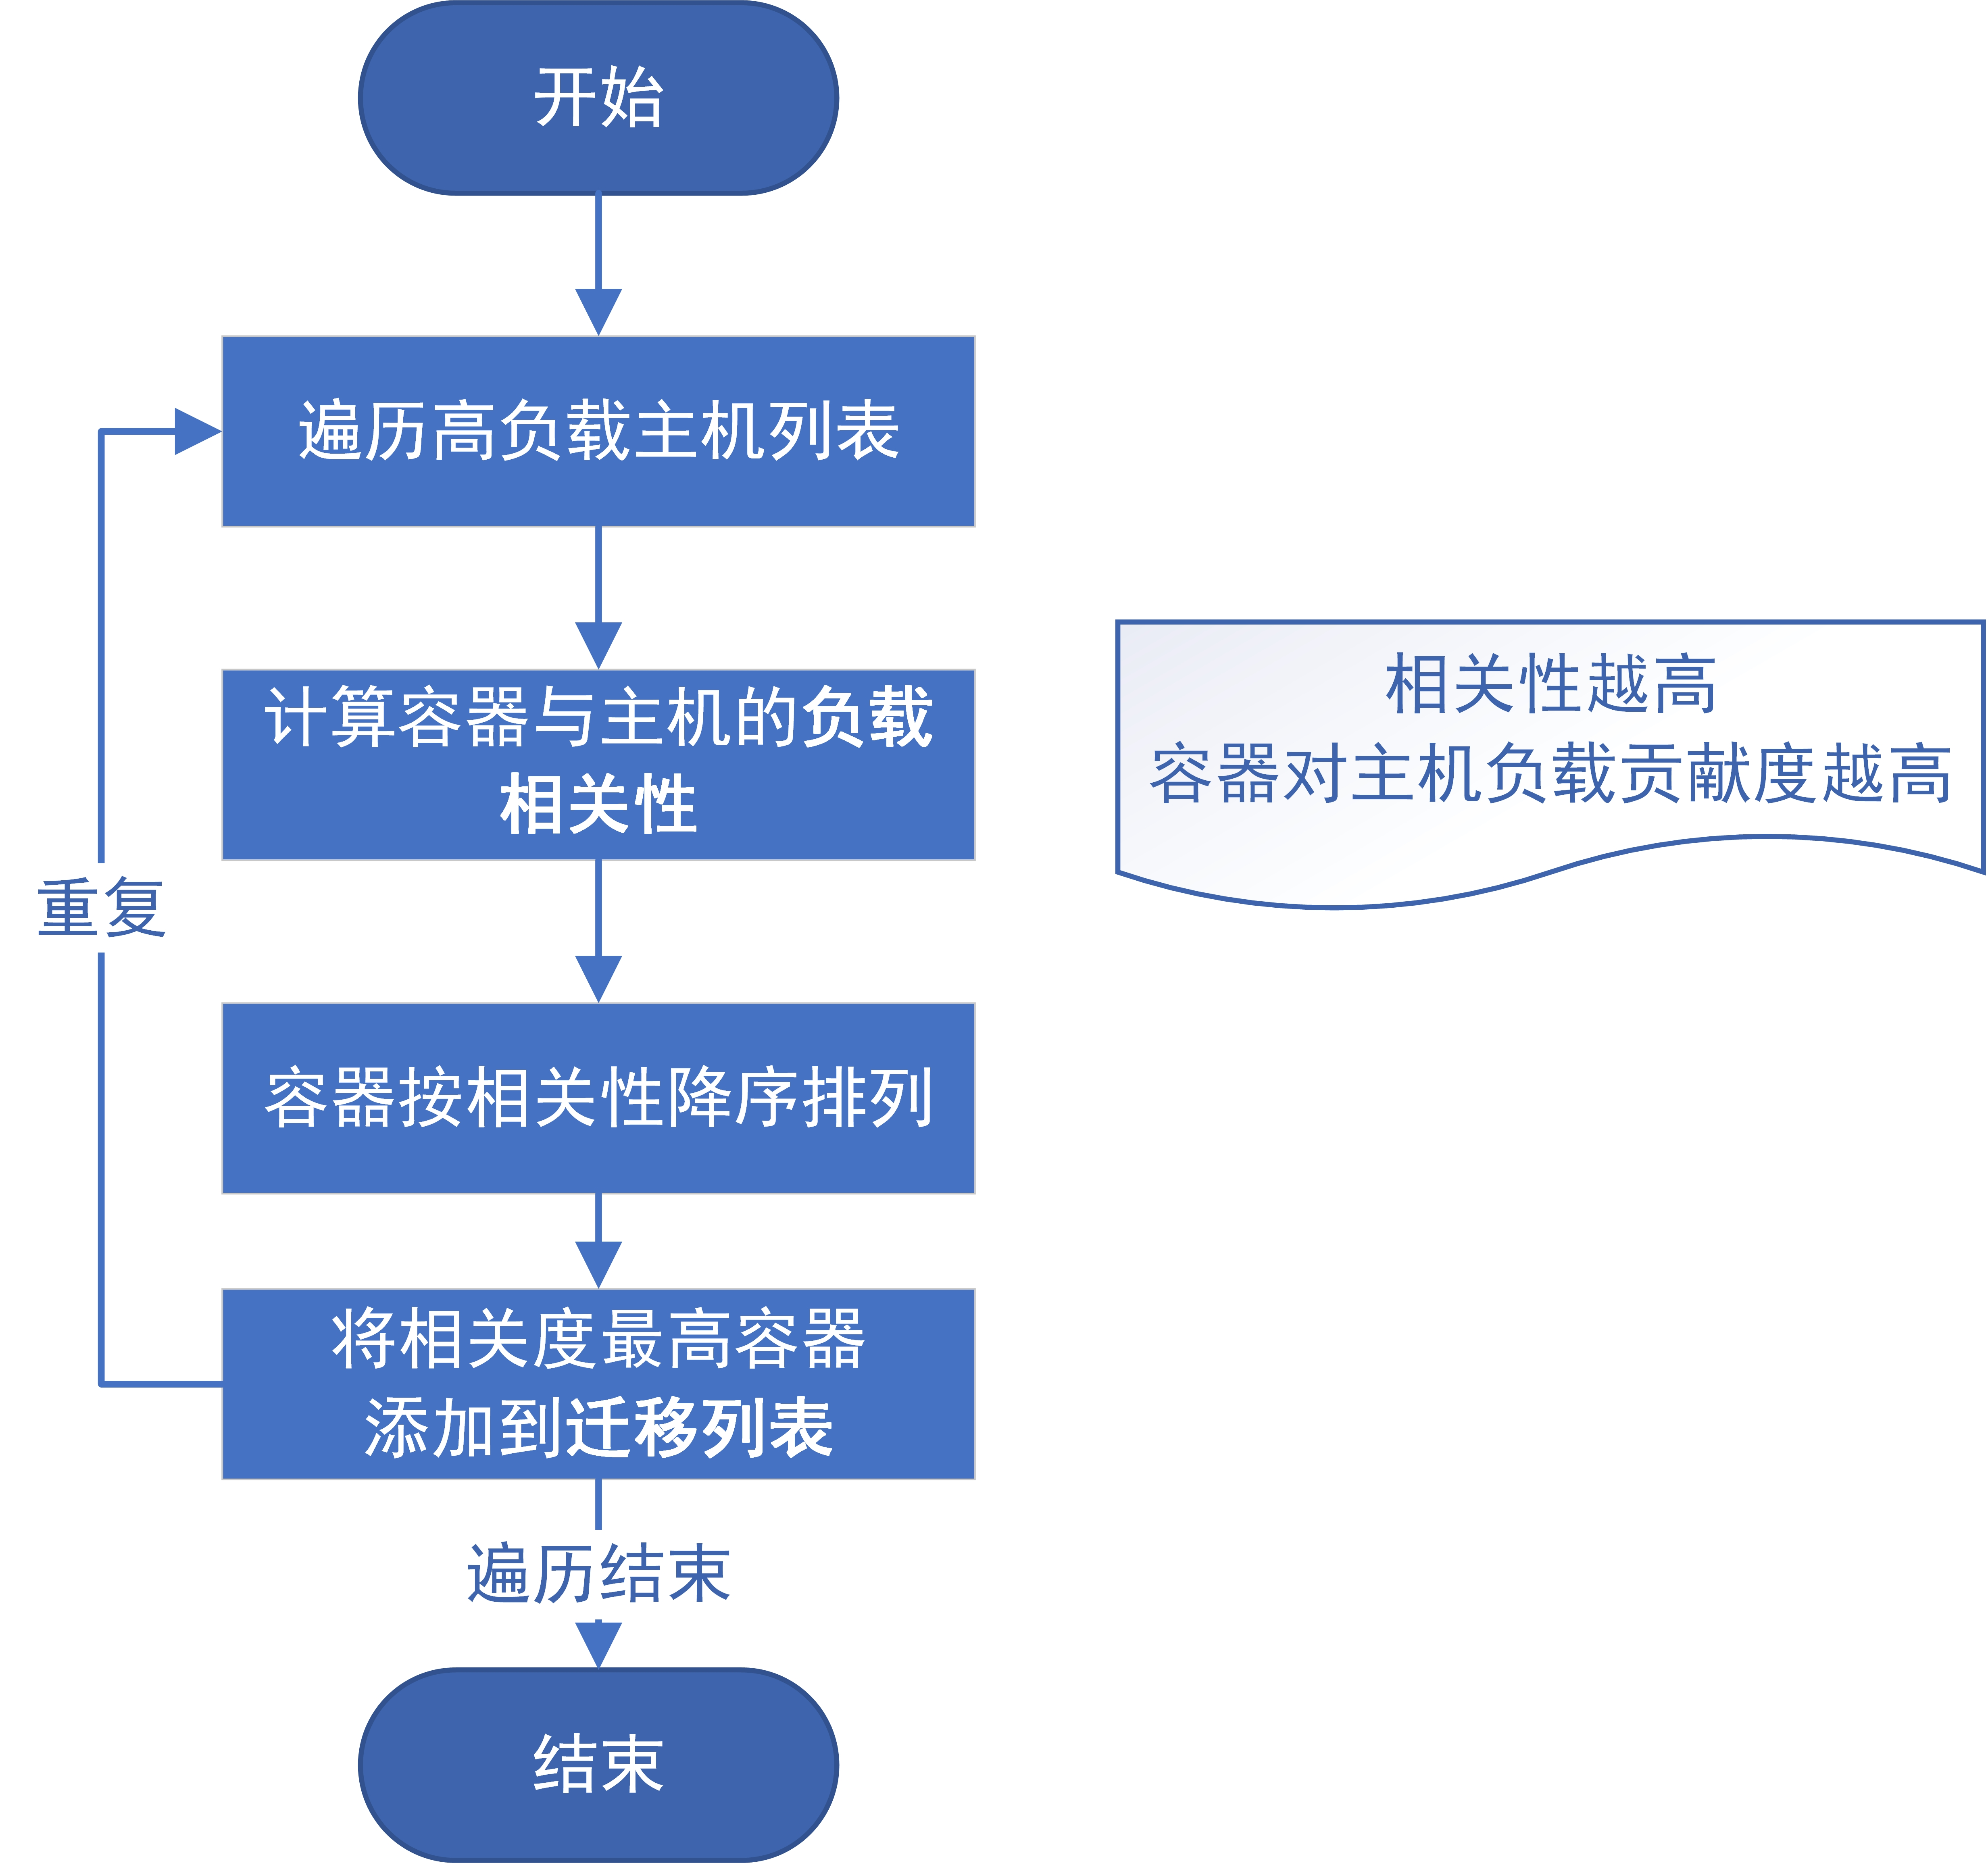
\includegraphics[width=0.52\textwidth]{figures/fig_4_1.jpg}
    \caption{容器选择算法流程}
    \label{fig:fig_4_1}
\end{figure}
\bigskip
\end{frame}

\begin{frame}
\frametitle{调度算法}
\framesubtitle{容器调度模块(1/3):主机选择算法 - 选择容器迁移目的主机}
\begin{figure}[htb]
    \centering
    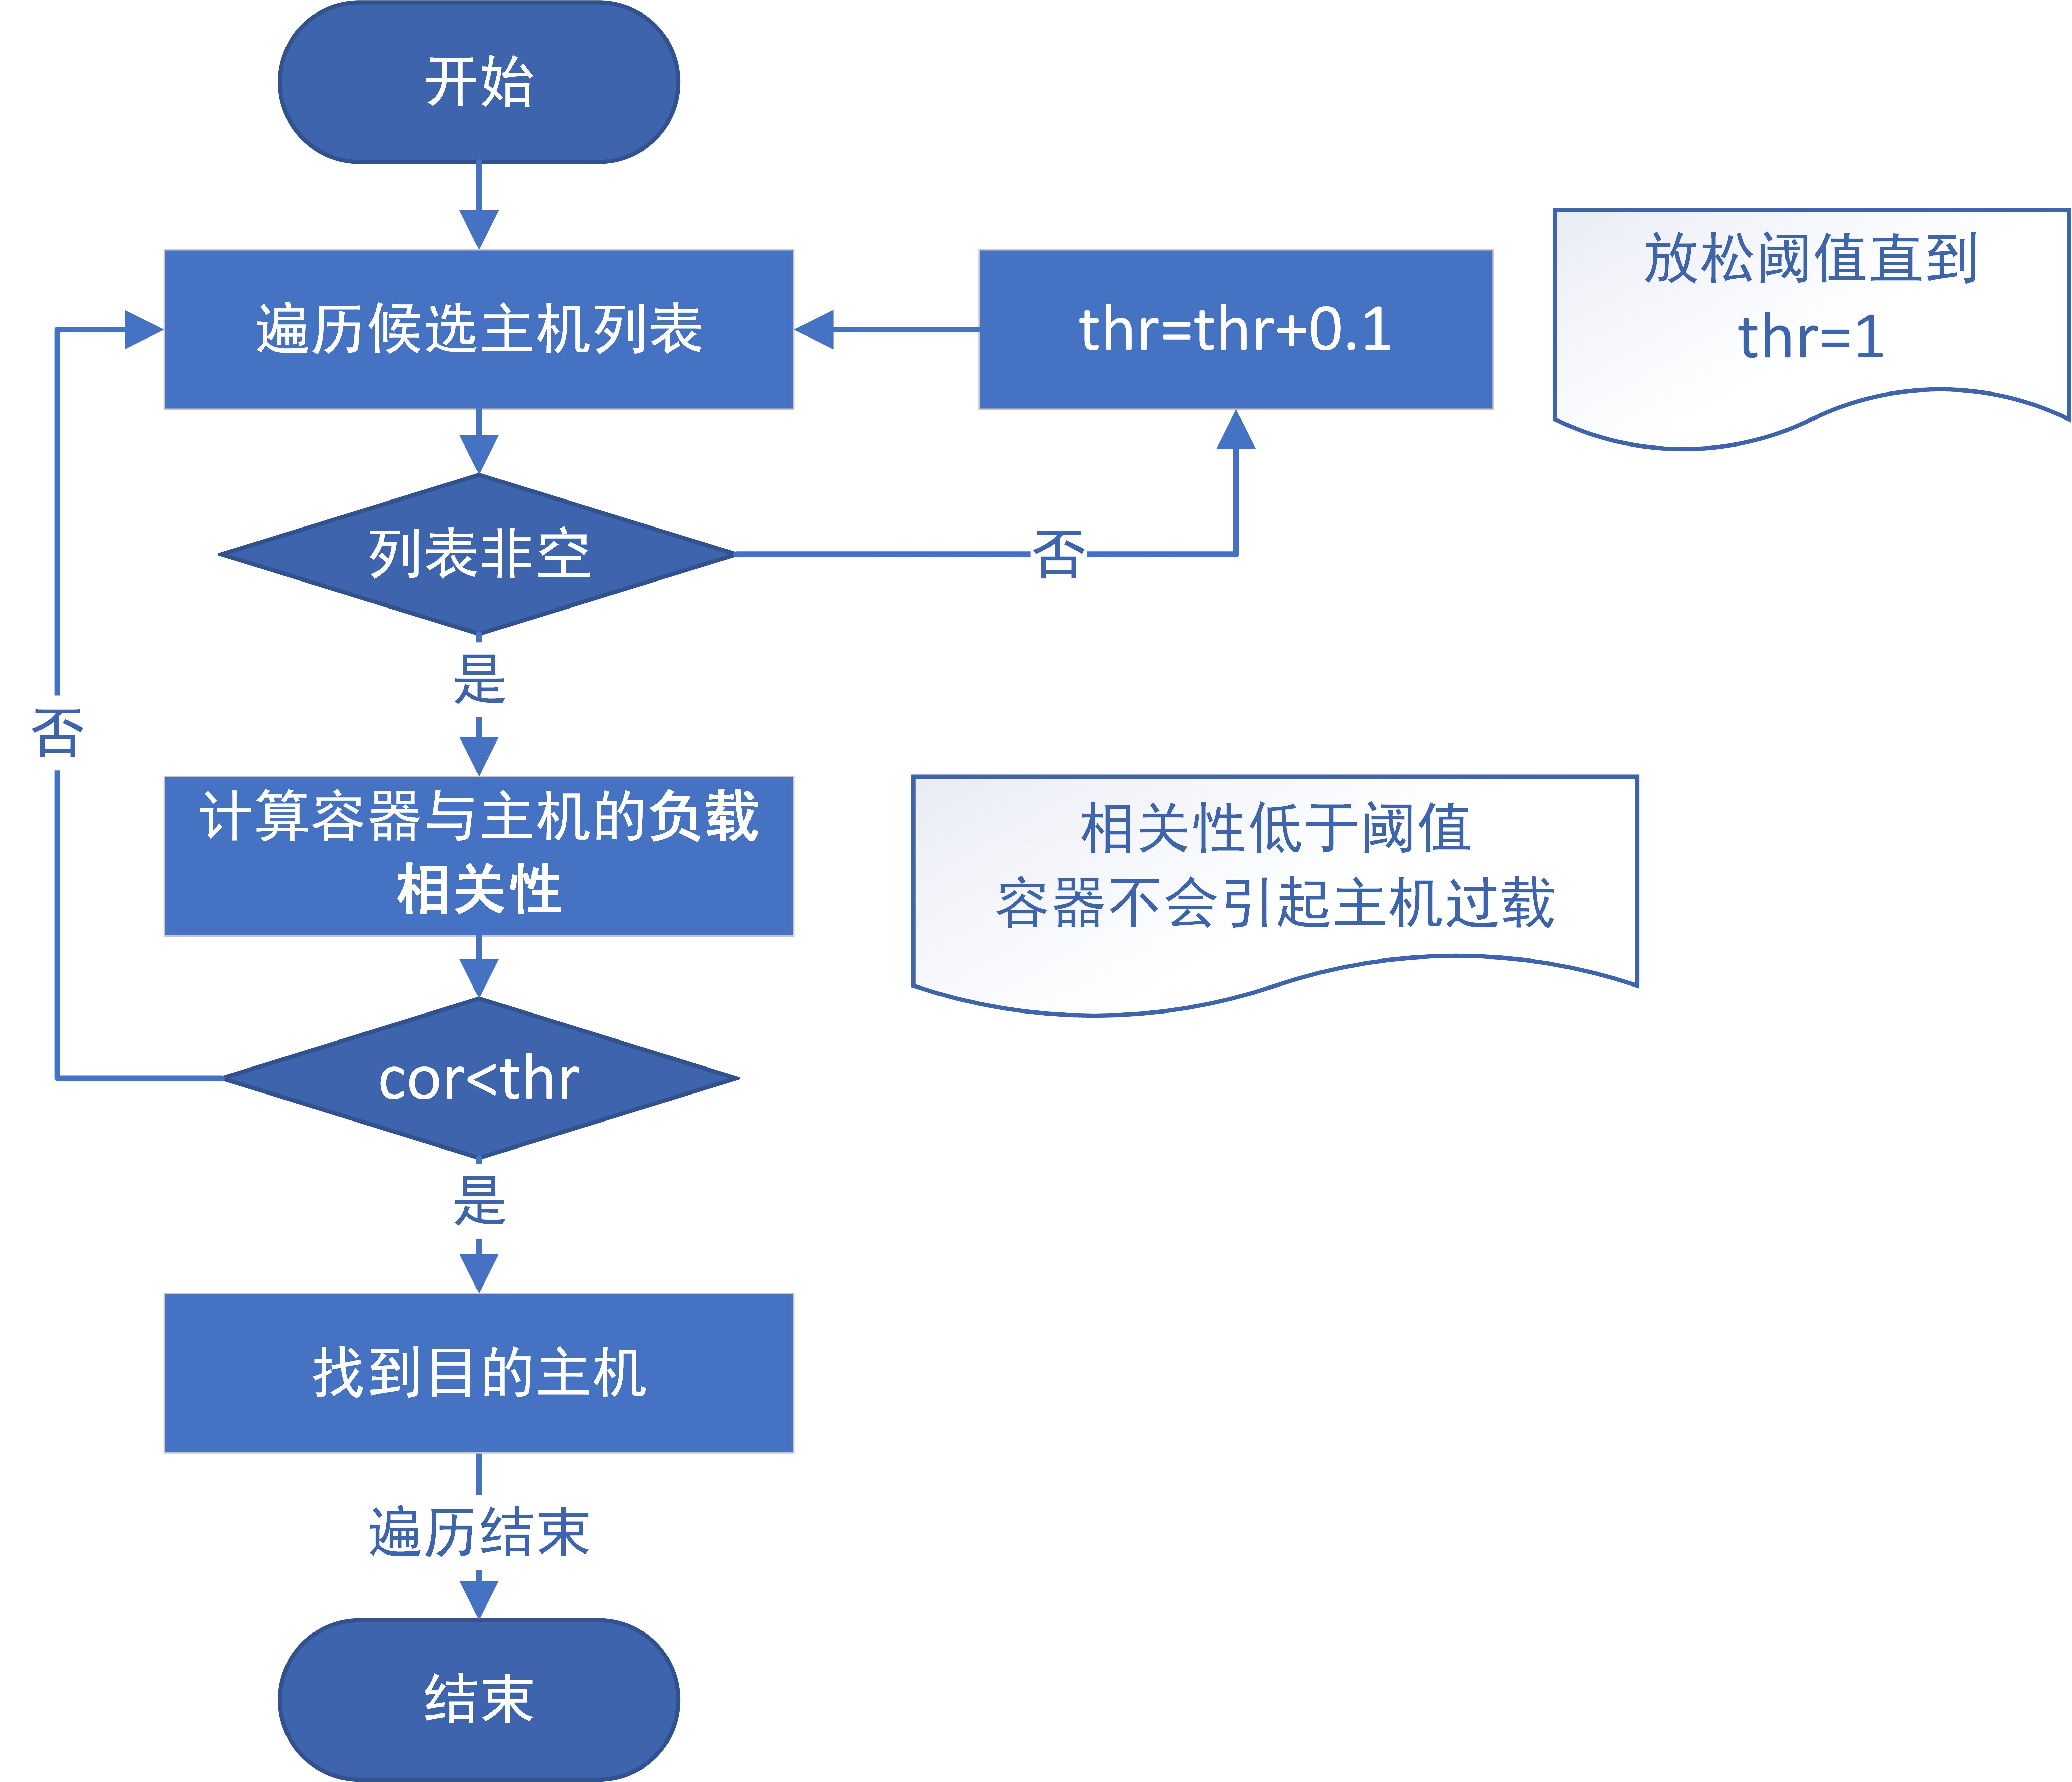
\includegraphics[width=0.58\textwidth]{figures/fig_4_2.jpg}
    \caption{主机选择算法流程}
    \label{fig:fig_4_2}
\end{figure}
\bigskip
\end{frame}

\begin{frame}
\frametitle{调度算法}
\framesubtitle{容器调度模块(2/3):容器迁移和放置算法 - 迁移高负载主机上容器、放置新增容器}
\begin{figure}[htb]
    \centering
    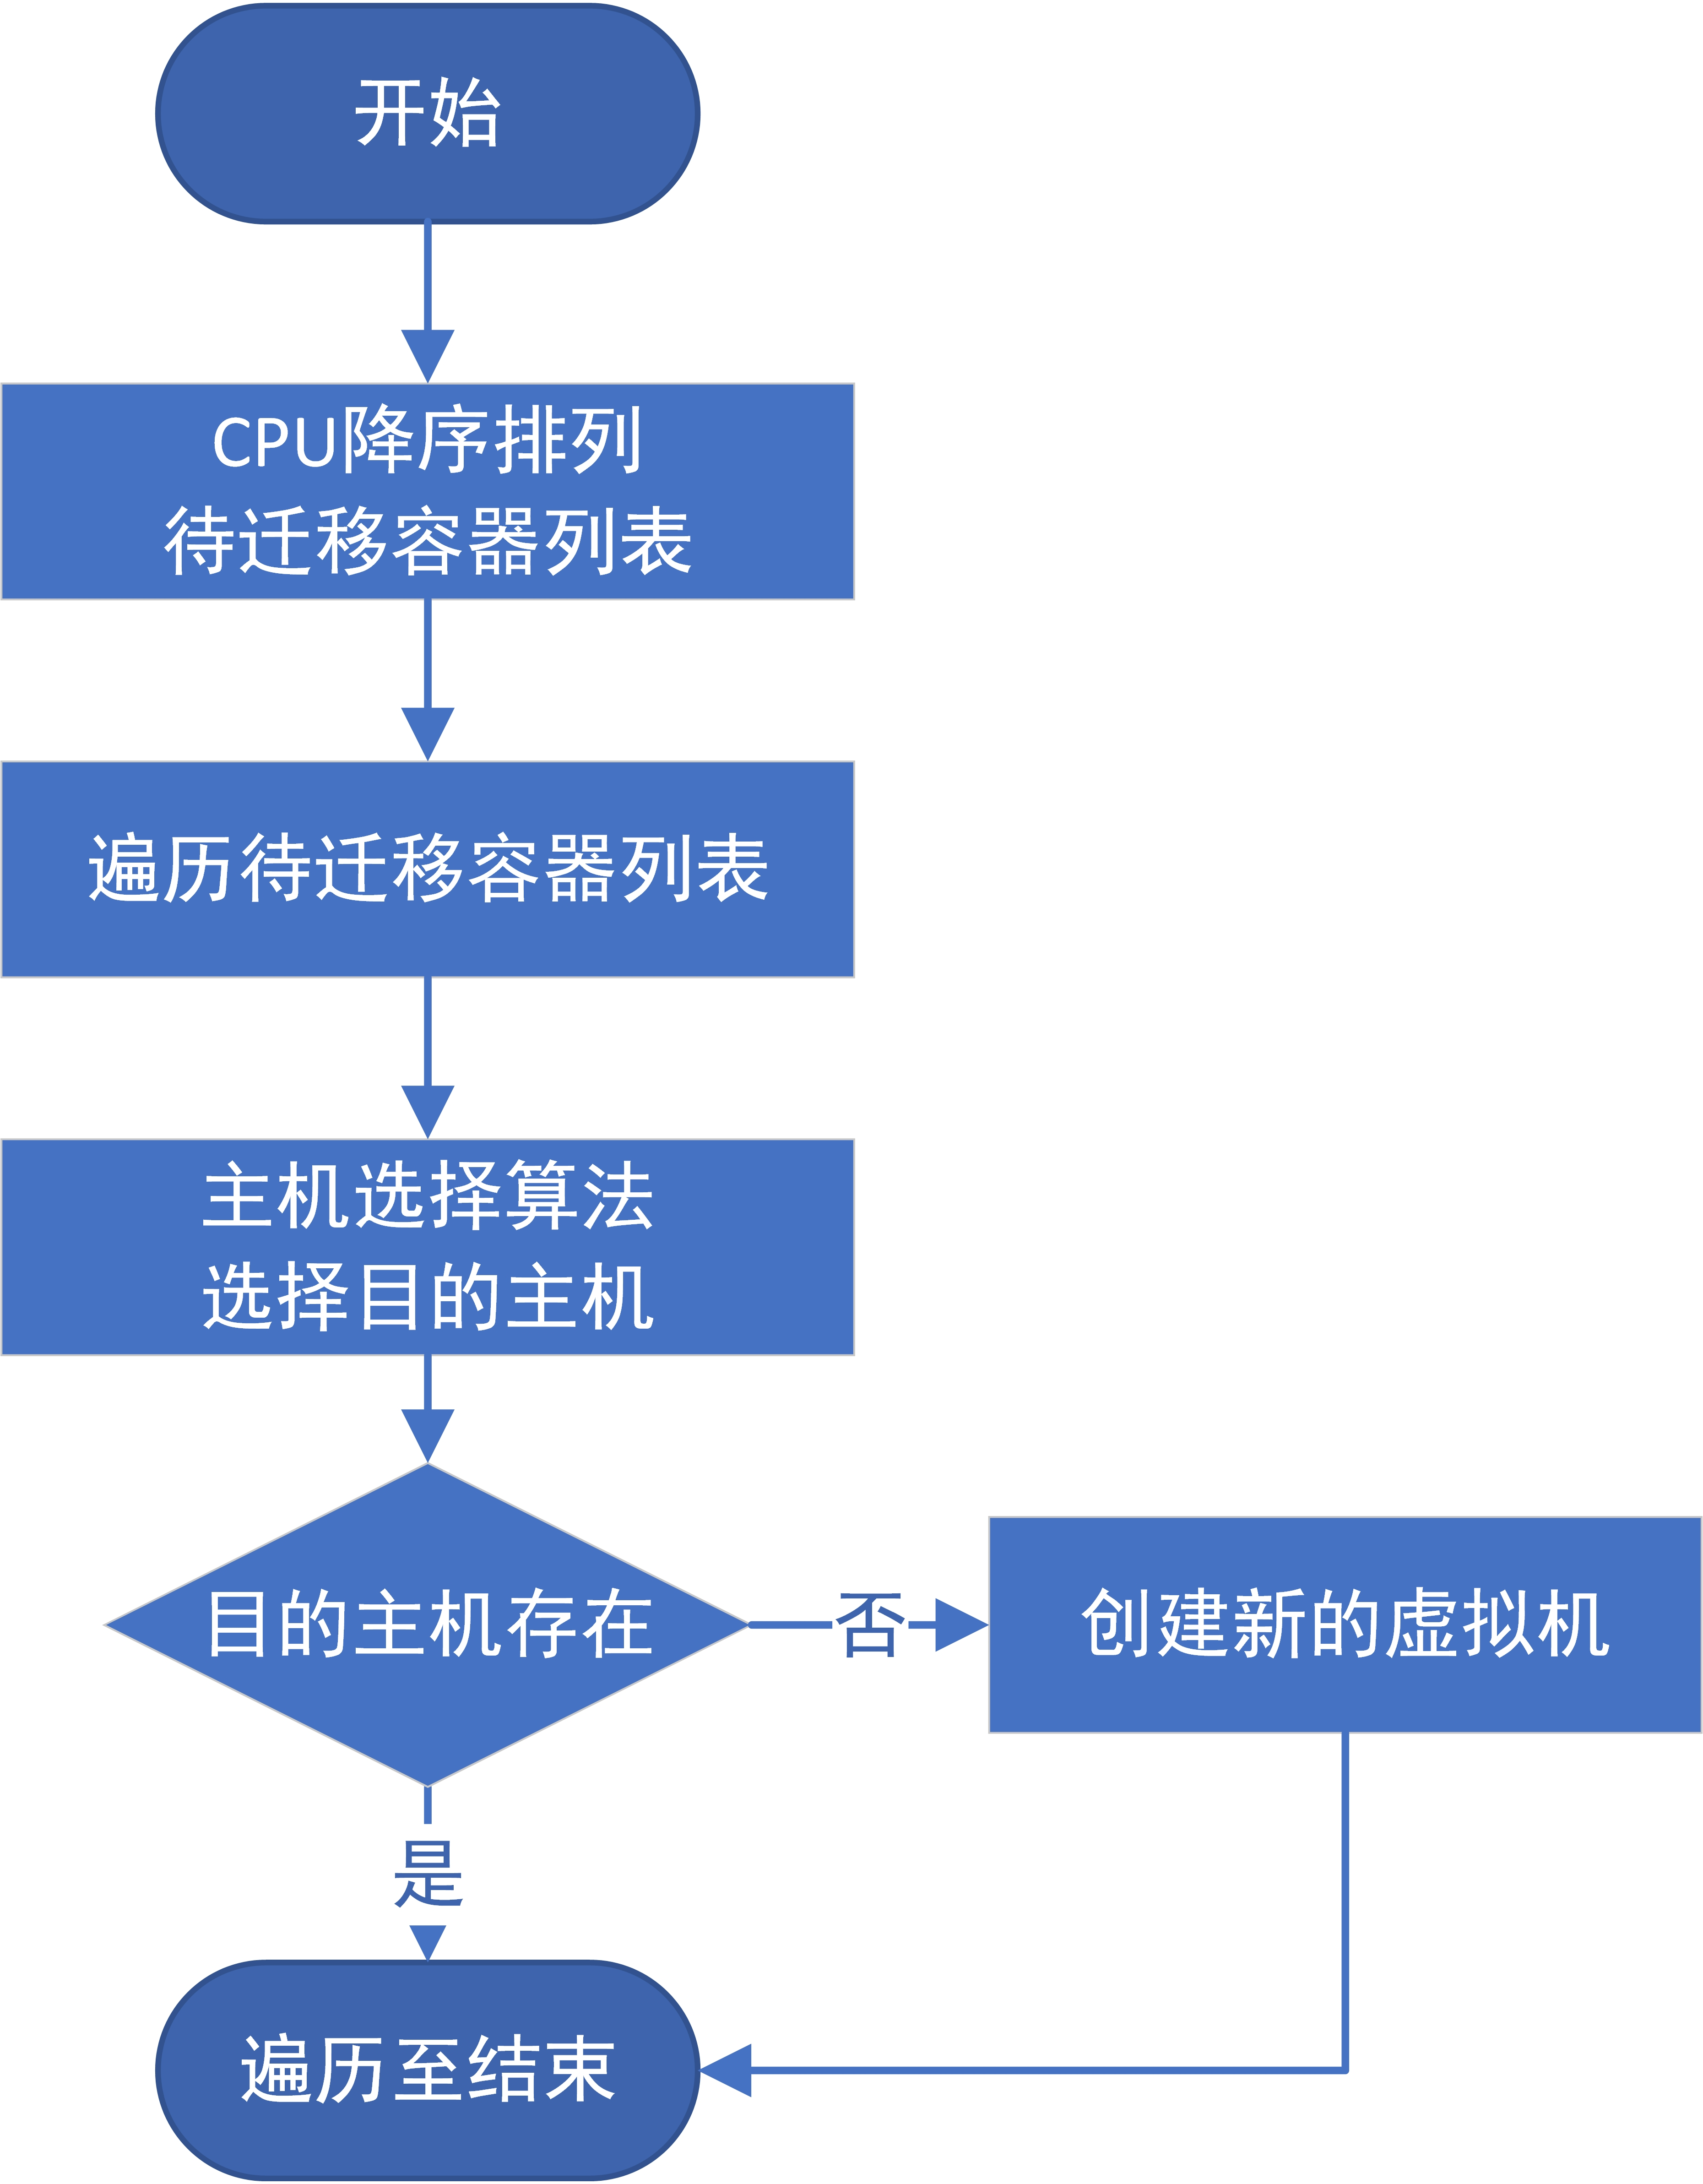
\includegraphics[width=0.4\textwidth]{figures/fig_4_3.jpg}
    \caption{容器迁移和放置算法流程}
    \label{fig:fig_4_3}
\end{figure}
\end{frame}

\begin{frame}
\frametitle{调度算法}
\framesubtitle{容器调度模块(3/3):容器合并算法 - 合并低负载主机容器}
\begin{figure}[htb]
    \centering
    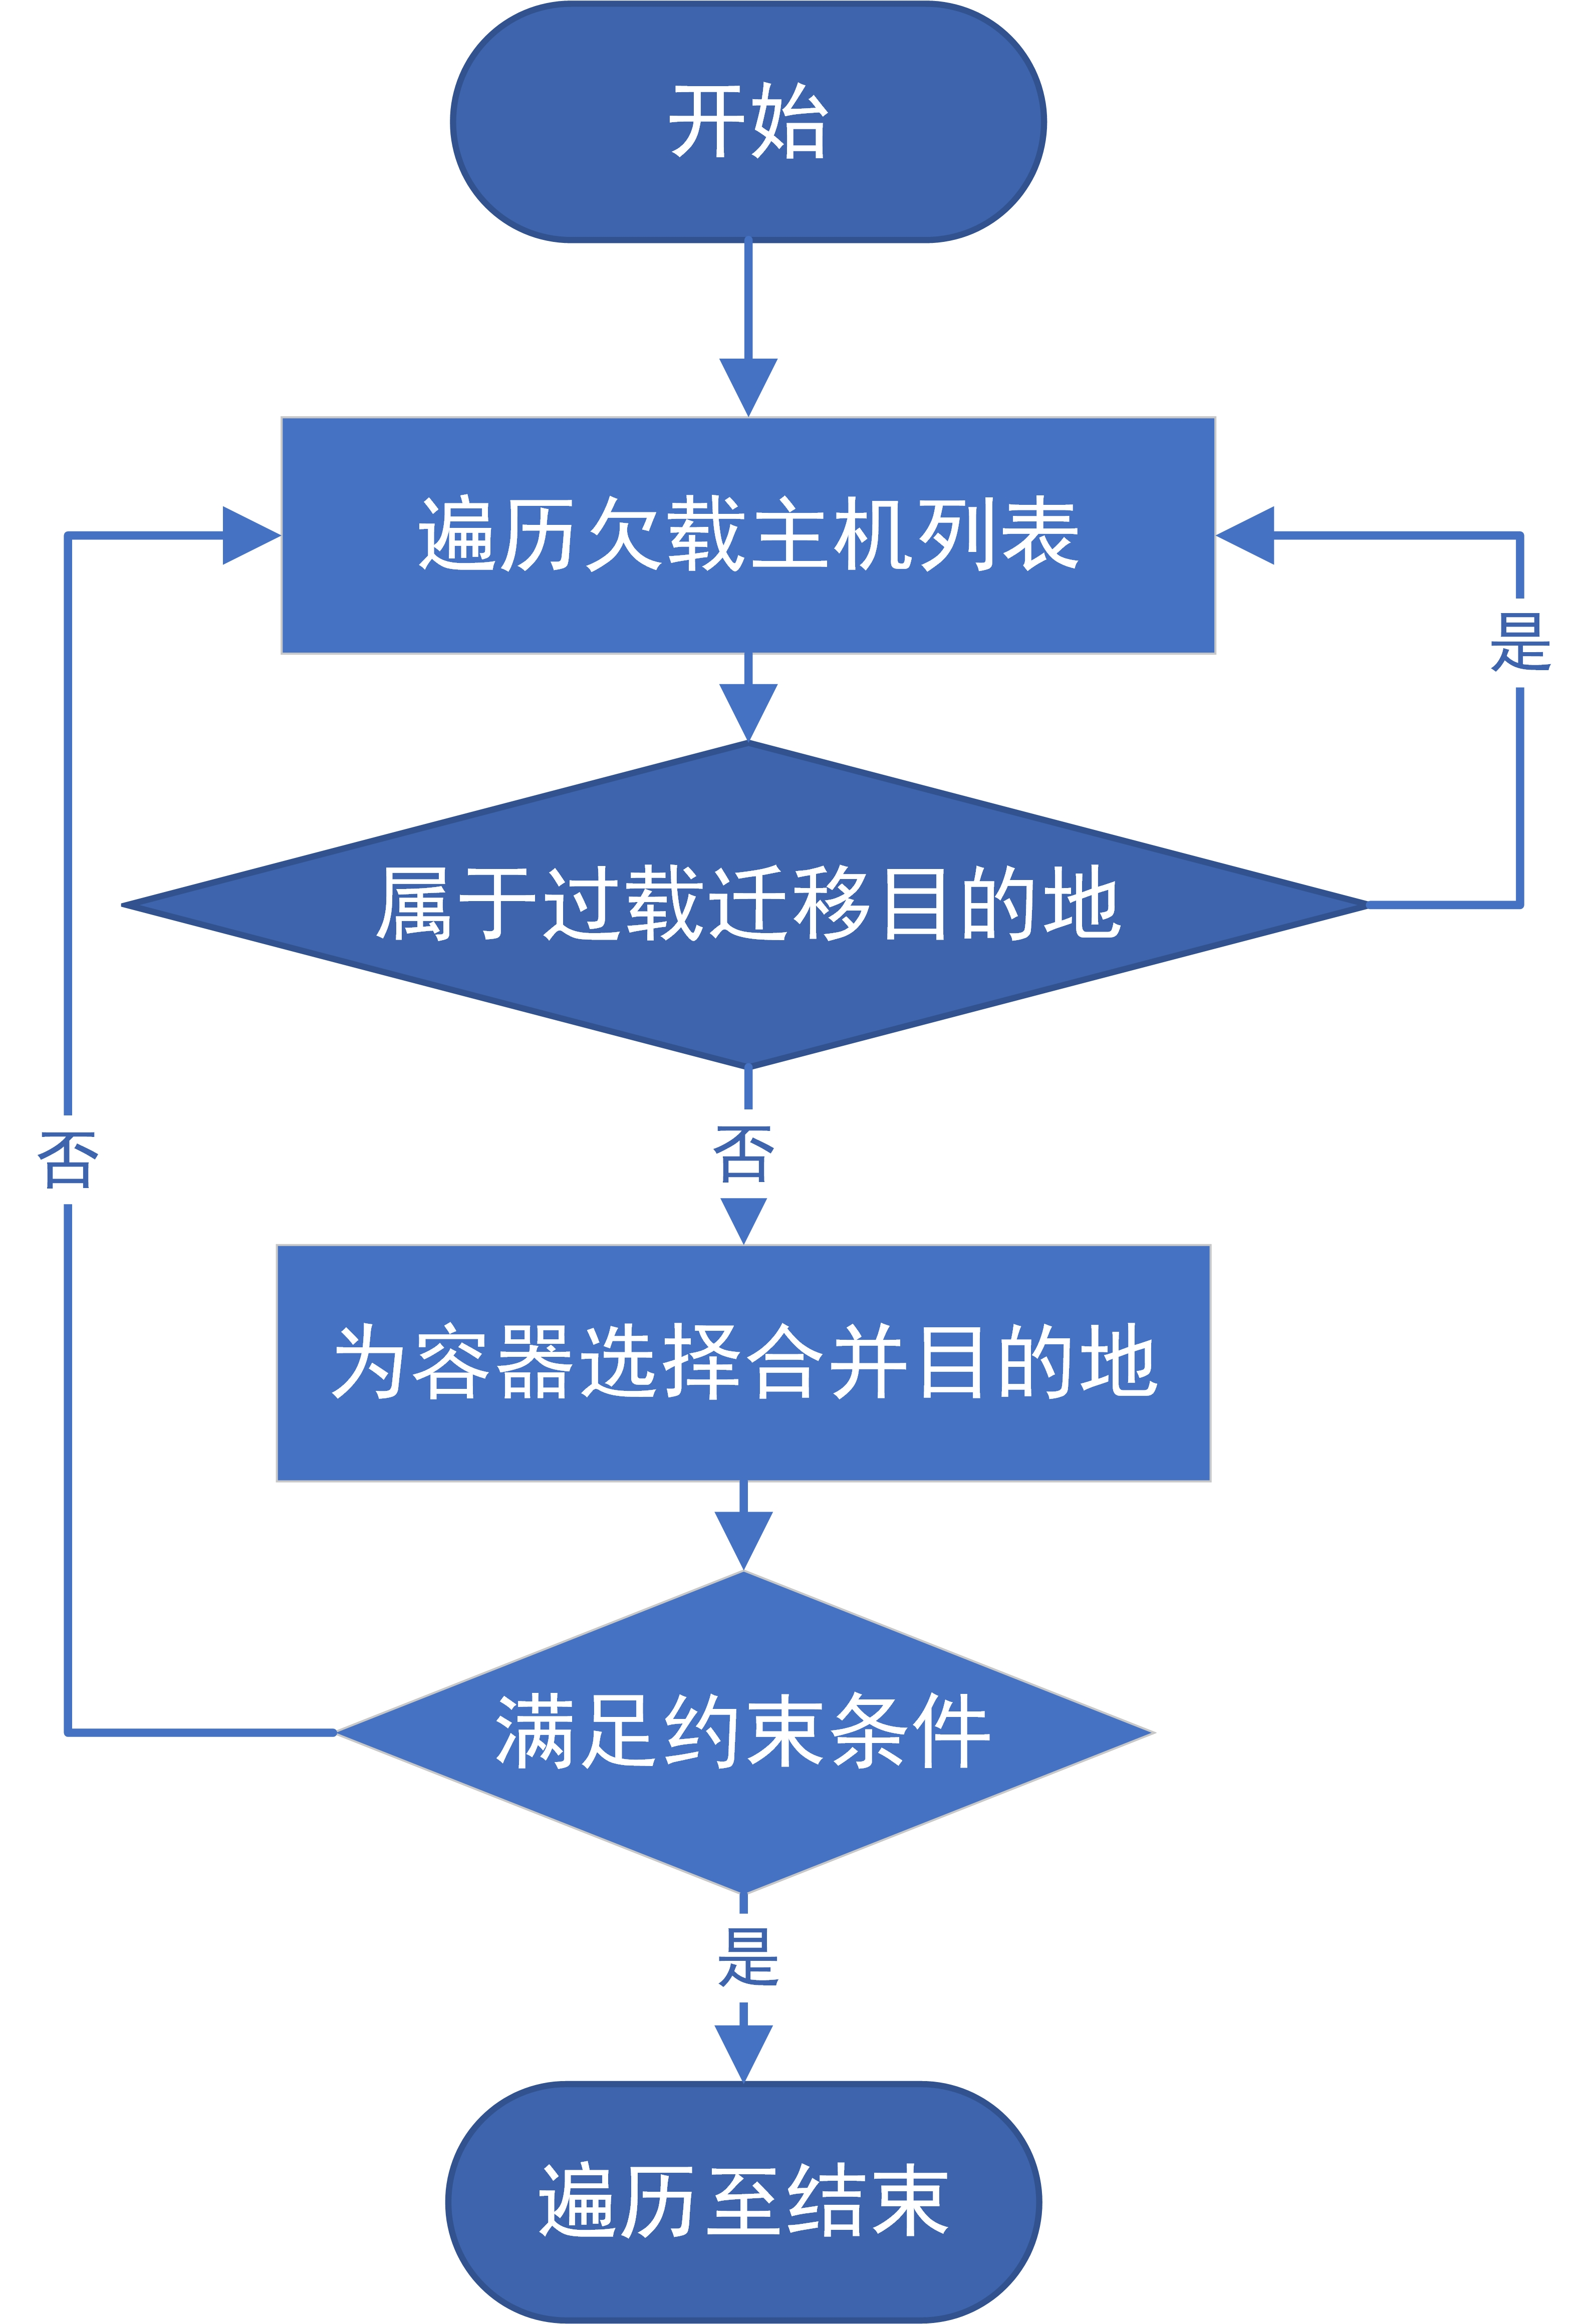
\includegraphics[width=0.36\textwidth]{figures/fig_4_4.jpg}
    \caption{容器合并算法流程}
    \label{fig:fig_4_4}
\end{figure}
\end{frame}

\subsection{实验结果与分析}

\begin{frame}
\frametitle{实验结果与分析}
\framesubtitle{QoS指标}
\begin{itemize}
    \item SLA违反率:容器未分配的CPU资源量在总请求量中的占比
    \begin{equation}
    \begin{align*}
        &SLA = \sum_{i=1}^{N_s}\sum_{j=1}^{N_{vm}}\sum_{p=1}^{N_v}
        \frac{CPU_r(vm_{ji},t_p) - CPU_a(vm_{ji},t_p)}{CPU_r(vm_{ji},t_p)} \\
        &\begin{cases}
            CPU_r(vm_{ji},t_p) = \sum_{k=1}^{N_c^{ji}}CPU_r(c_{kji},t_p) \\
            CPU_a(vm_{ji},t_p) = \sum_{k=1}^{N_c^{ji}}CPU_a(c_{kji},t_p)
        \end{cases}
    \end{align*}
    \end{equation}
    \item 容器对CPU资源的请求量:依据\textbf{超量因子}$P_n$从历史记录中获取
        \begin{enumerate}
            \item 从容器负载历史记录中选择一个负载值 $L_{per}$
            \item 概率 $P(L \le L_{per}) \ge P_n$
            \item $min(L_{per})$ 即为容器对CPU资源的请求量
        \end{enumerate}
\end{itemize}
\end{frame}

\begin{frame}
\frametitle{实验结果与分析}
\framesubtitle{实验设置}
\begin{itemize}
    \item 容器负载数据(PlanetLab)、服务器和虚拟机配置、CloudSim
    \item 对比算法
    \begin{itemize}
        \item \textbf{FFHS(Kubernetes)}:选择第一台满足资源请求的主机
        \item \textbf{LFHS}:FFHS基础上增加主机CPU降序排列预处理
        \item \textbf{WEEC}:聚类划分容器,基于能耗特征的启发式算法
        \item \textbf{本文基于动态伸缩的容器调度策略}
    \end{itemize}
    \item 对照实验:
    \begin{itemize}
        \item 控制容器伸缩的\textbf{"应用总体负载阈值"$=70\%$}
        \item CorHS中的\textbf{"负载相关度阈值"$=0.5$}
    \end{itemize}
    \begin{table}[hftb]
        \centering
        \resizebox{0.8\textwidth}{!}{%
            \begin{tabular}{ccccc}
                \toprule
                \textbf{实验组} & \textbf{约束目标} & \textbf{UL} & \textbf{OL} & \textbf{Overbooking}\\
                \midrule
                group.1 & OL阈值 & $70\%$ & $[80\%,90\%,100\%]$ & $80th$\\
                group.2 & UL阈值 & $[50\%,60\%,70\%]$ & $80\%$ & $80th$ \\
                group.3 & Overbooking阈值& $70\%$ & $80\%$ & $[20th,40th,80th]$\\
                \bottomrule
            \end{tabular}
        }
        \caption{实验对照组设置}
        \label{tab:tab5}
    \end{table}
\end{itemize}
\end{frame}

\begin{frame}
\frametitle{实验结果与分析}
\framesubtitle{实验结果:group.1 \textbf{UL=$70\%$ OL=$[80\%,90\%,100\%]$, Overbooking=$80th$}}
\begin{minipage}{\textwidth}
    \centering
    \begin{figure}[htb]
    \centering
    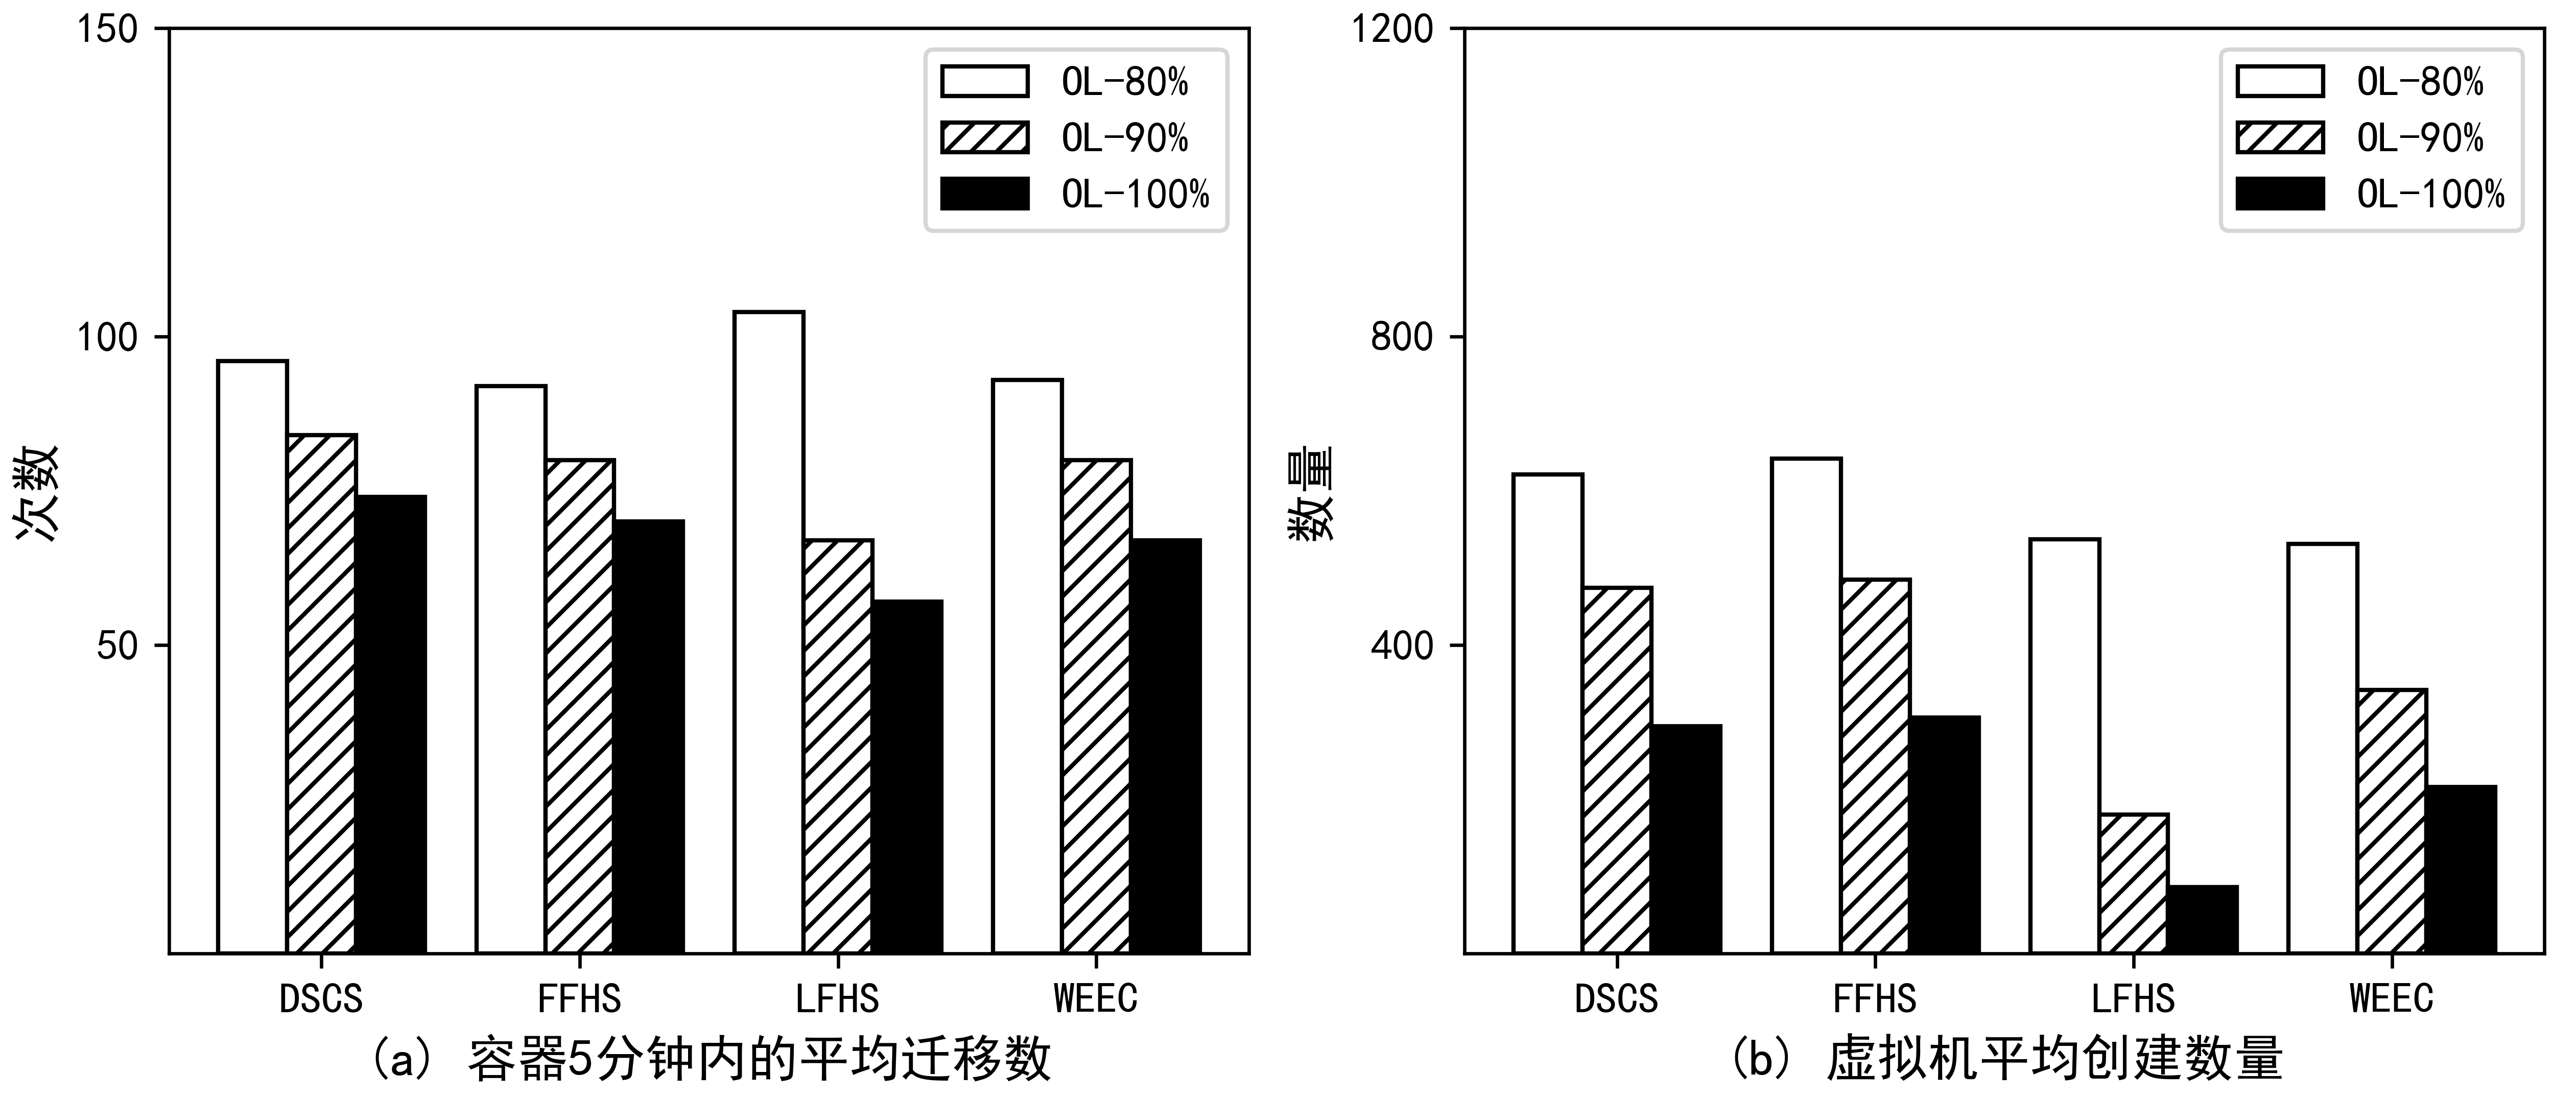
\includegraphics[width=0.45\textwidth]{figures/fig15_4-4_a.png}
    \end{figure}
\end{minipage}
\begin{minipage}{\textwidth}
    \centering
    \begin{figure}[htb]
    \centering
    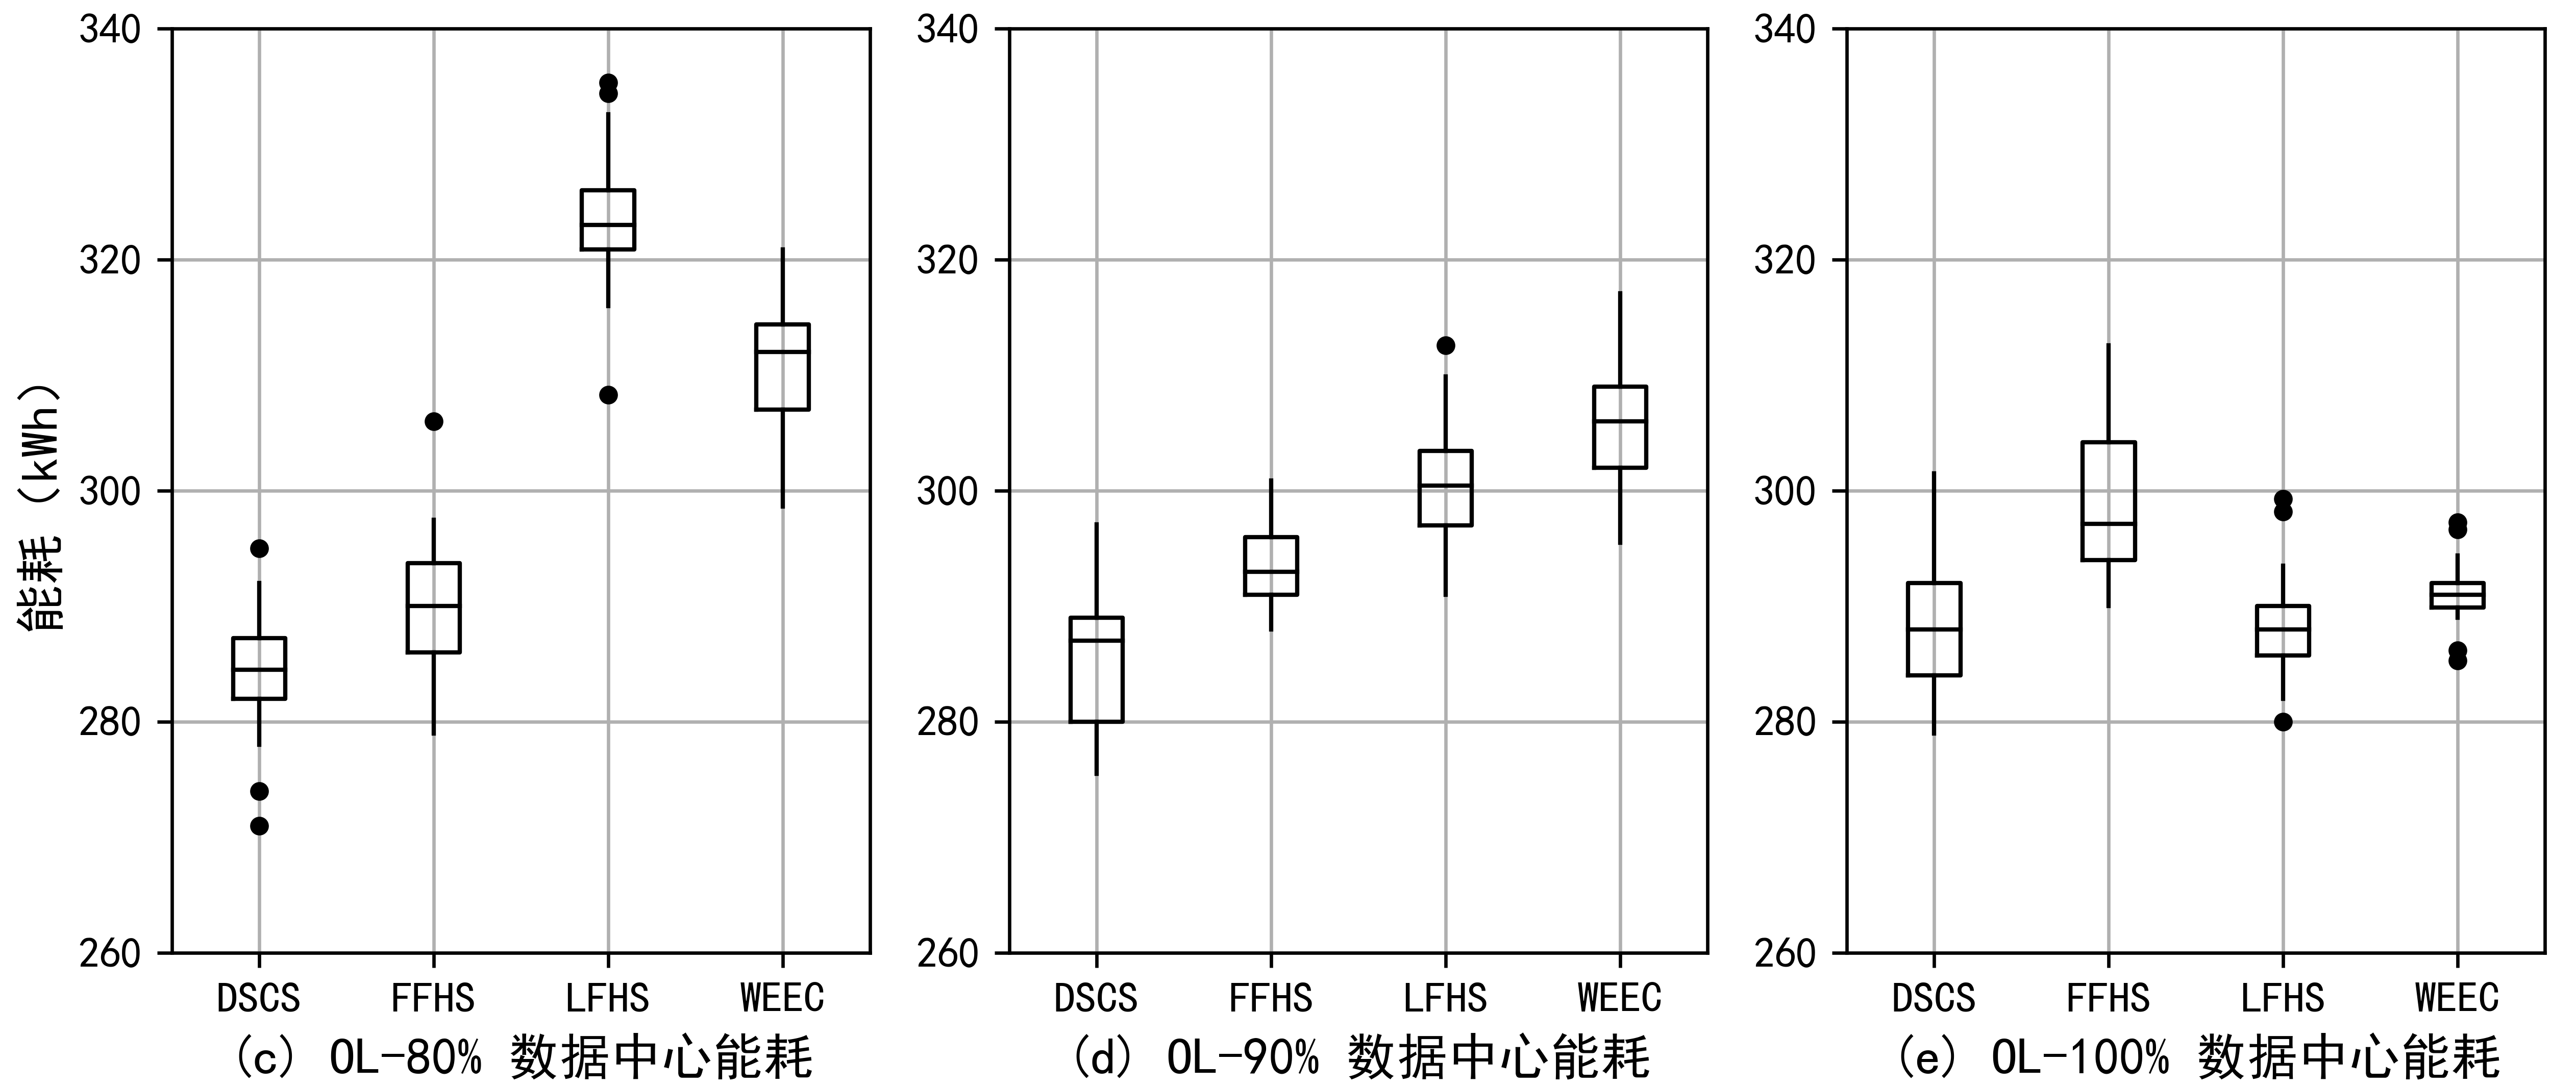
\includegraphics[width=0.45\textwidth]{figures/fig15_4-4_b.png}
    \end{figure}
\end{minipage}
\begin{minipage}{\textwidth}
    \centering
    \begin{figure}[htb]
    \centering
    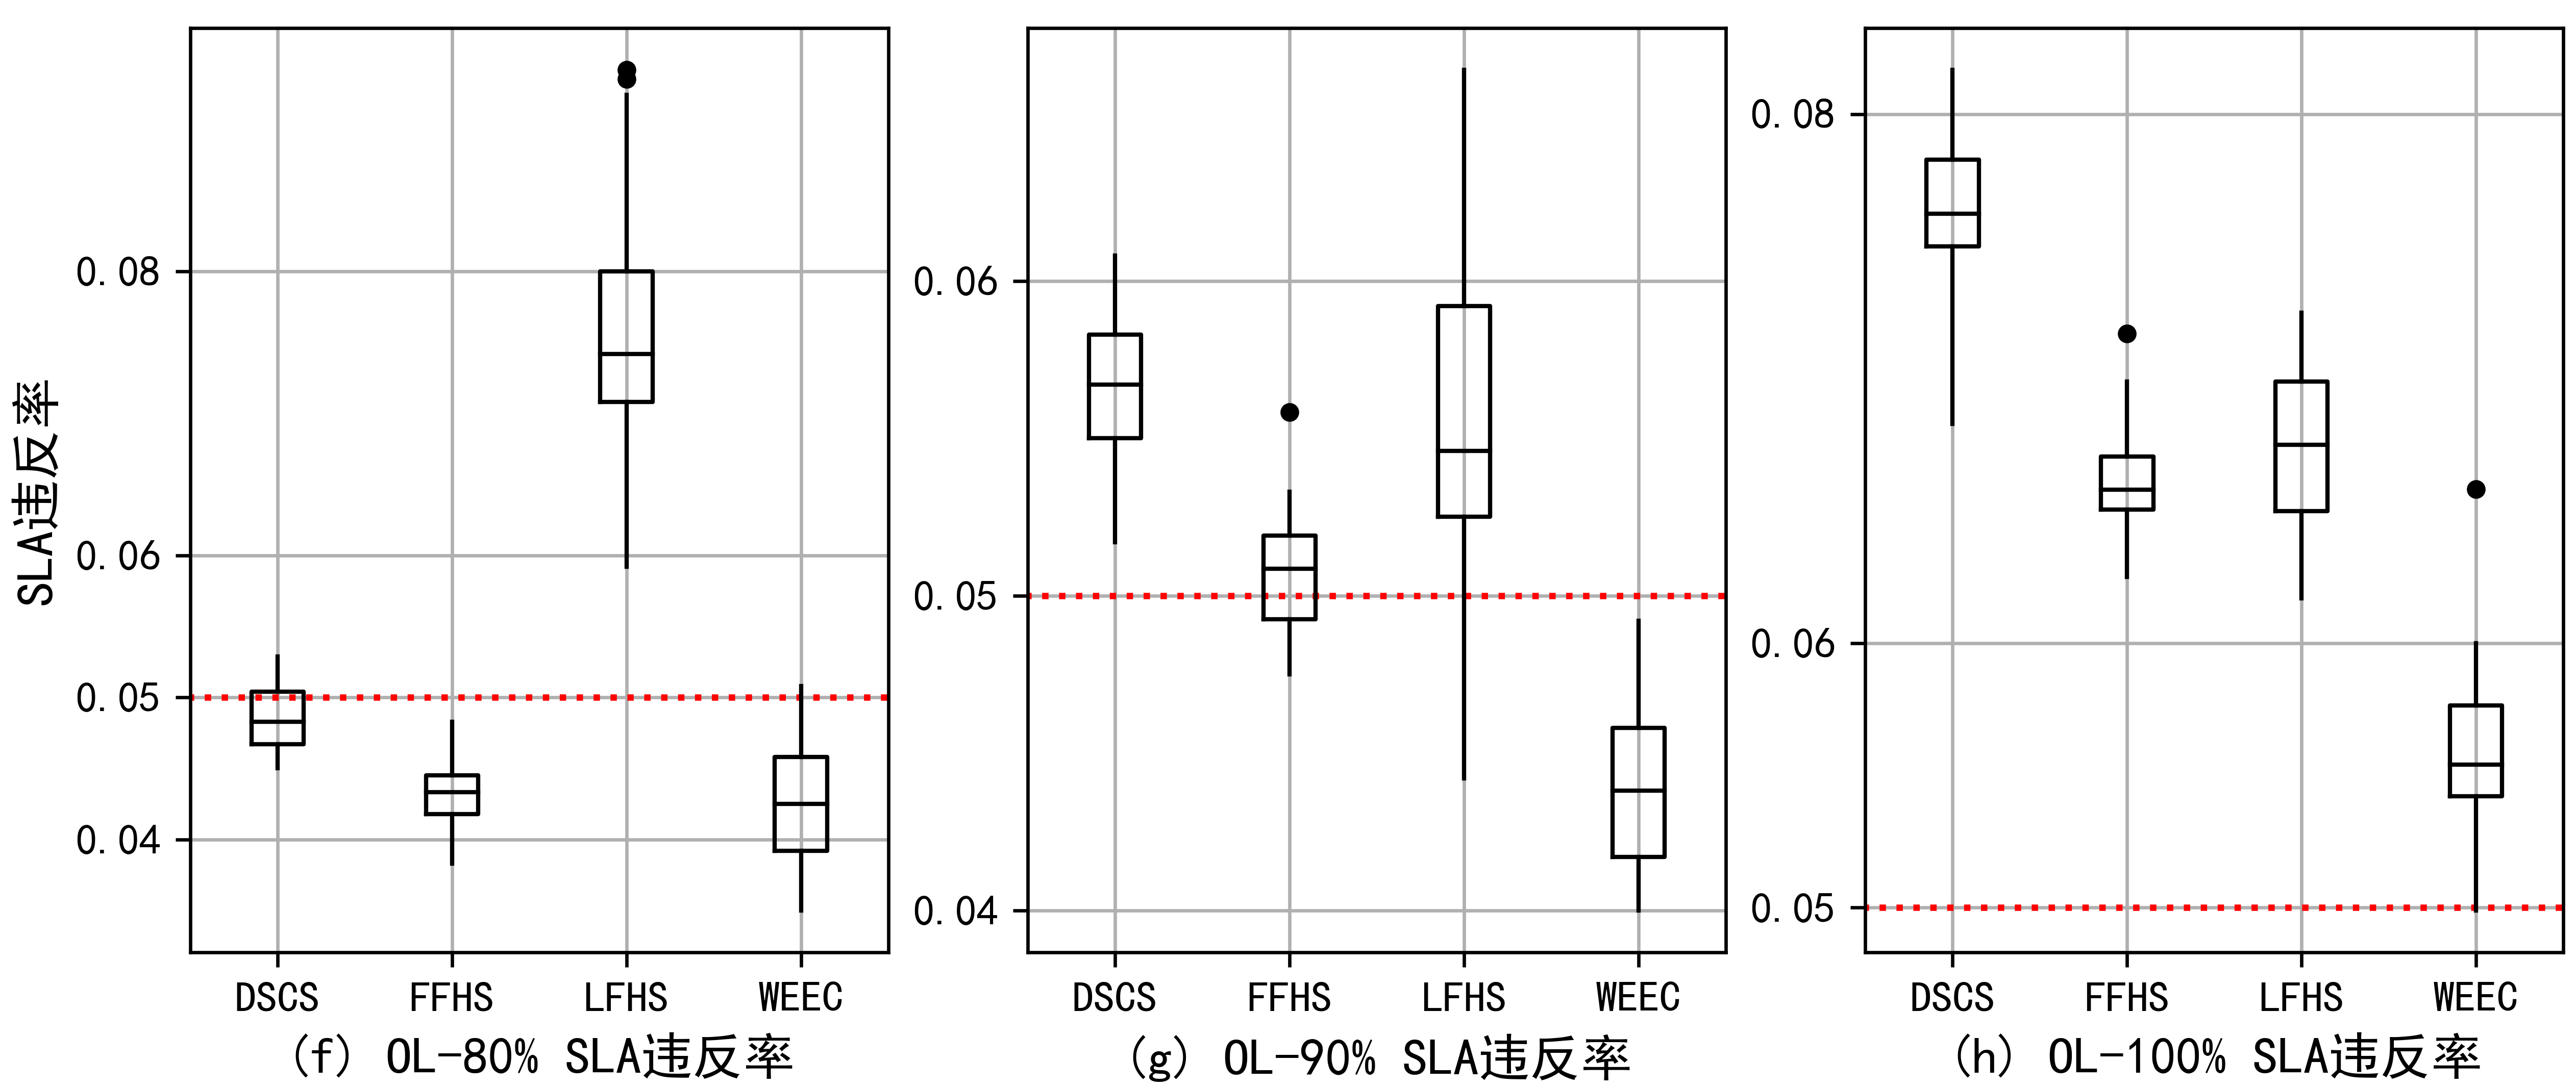
\includegraphics[width=0.45\textwidth]{figures/fig15_4-4_c.png}
    \caption{group.1 4种调度策略容器迁移、虚拟机创建数、能耗和SLA对比}
    \label{fig:fig15}
    \end{figure}
\end{minipage}
\end{frame}

\begin{frame}
\frametitle{实验结果与分析}
\framesubtitle{实验结果:group.2 \textbf{UL=$[50\%,60\%,70\%]$ OL=$80\%$, Overbooking=$80th$}}
\begin{minipage}{\textwidth}
    \centering
    \begin{figure}[htb]
    \centering
    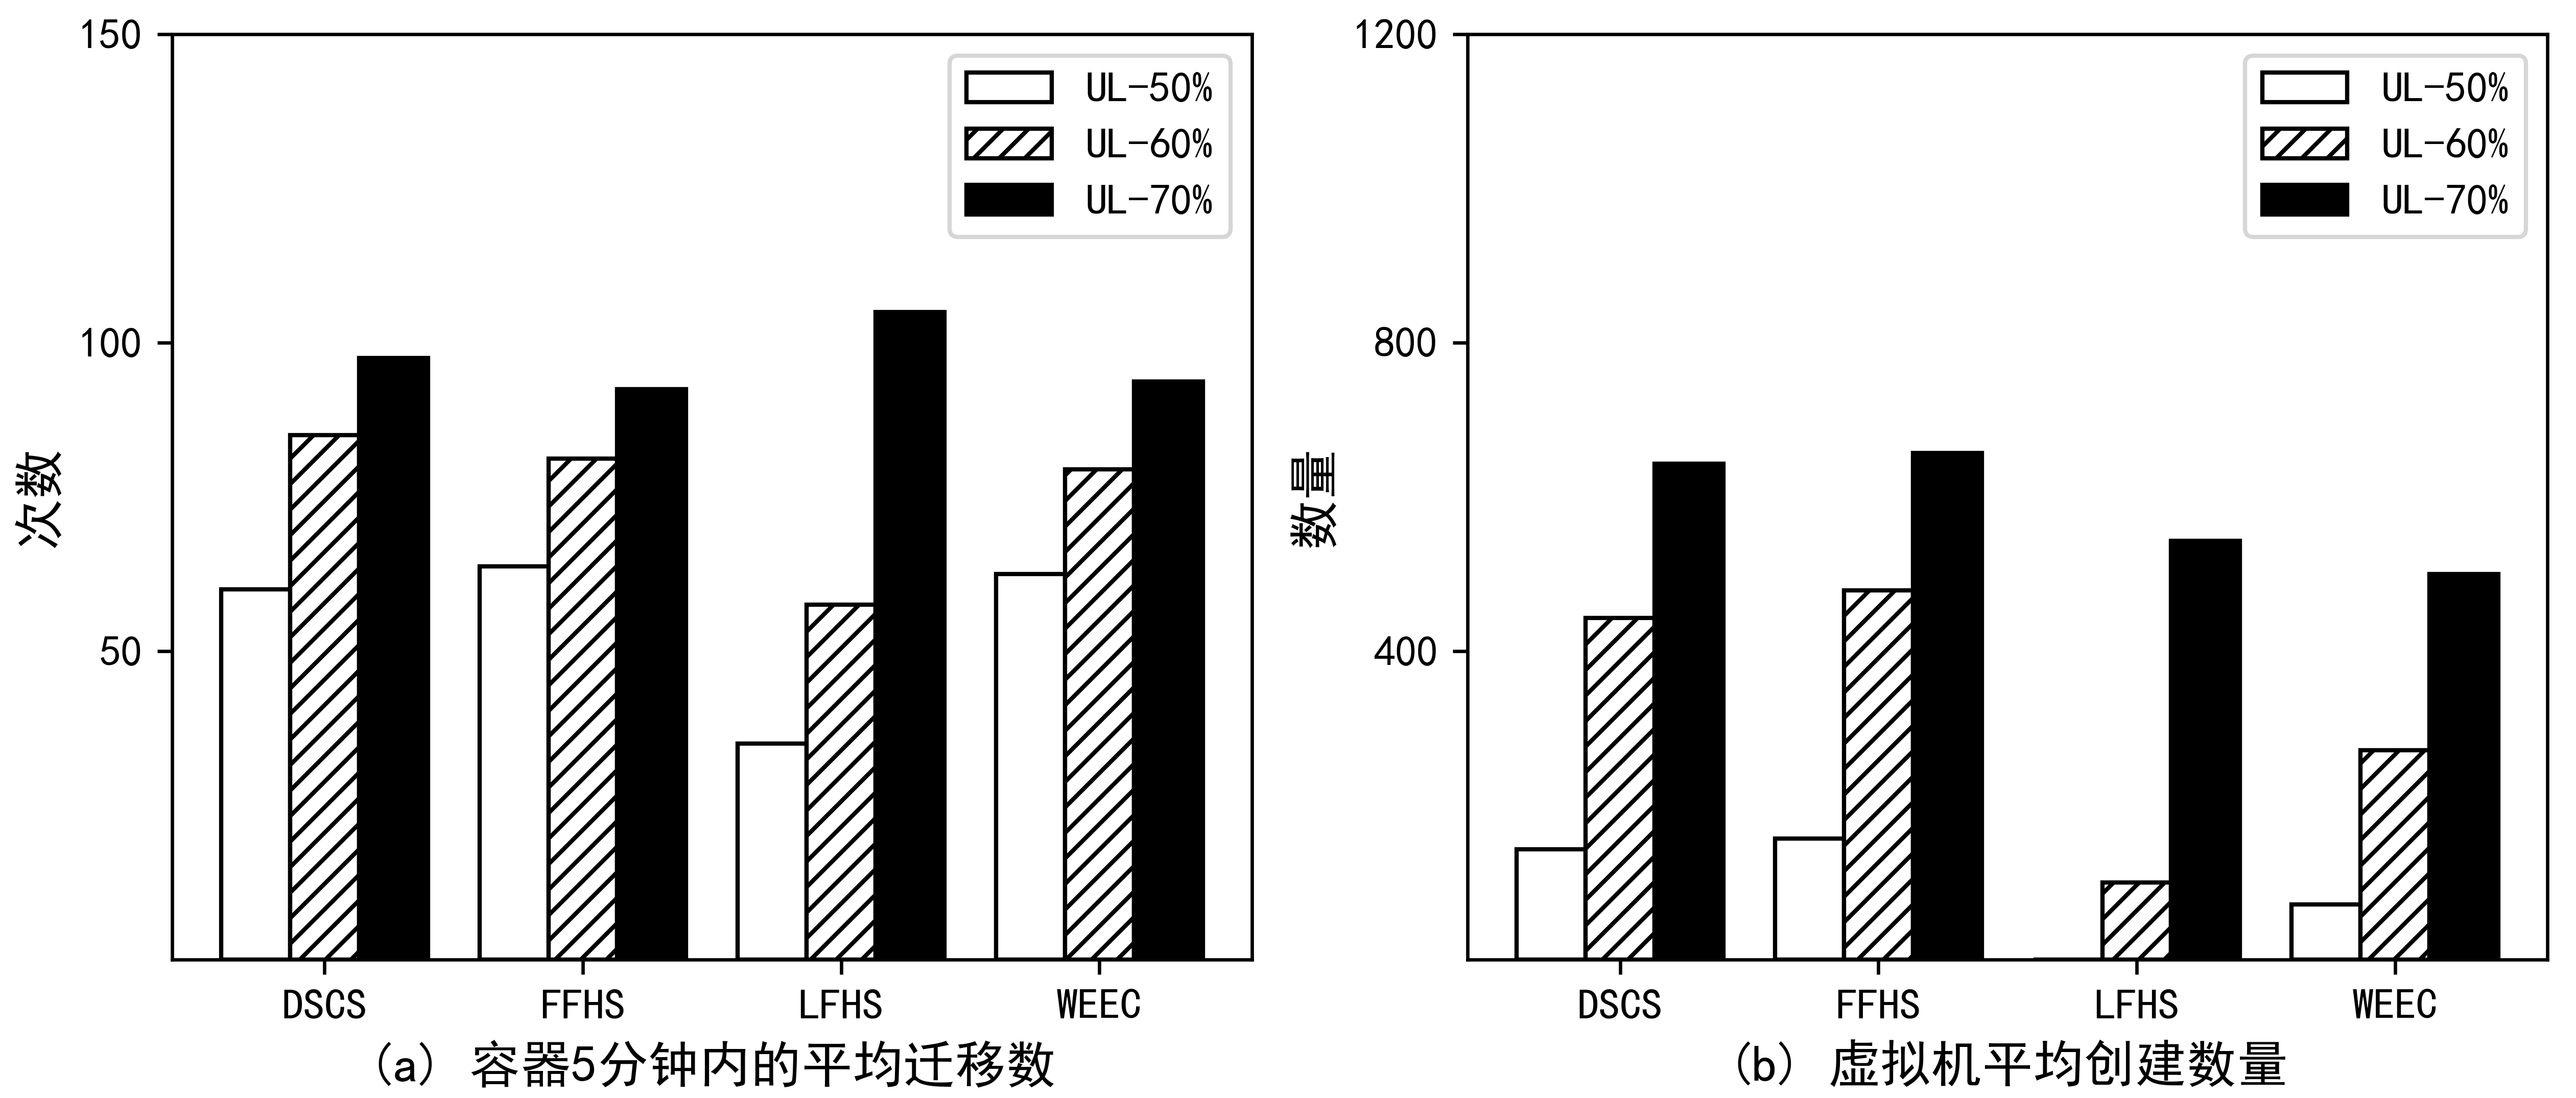
\includegraphics[width=0.45\textwidth]{figures/fig16_4-5_a.png}
    \end{figure}
\end{minipage}
\begin{minipage}{\textwidth}
    \centering
    \begin{figure}[htb]
    \centering
    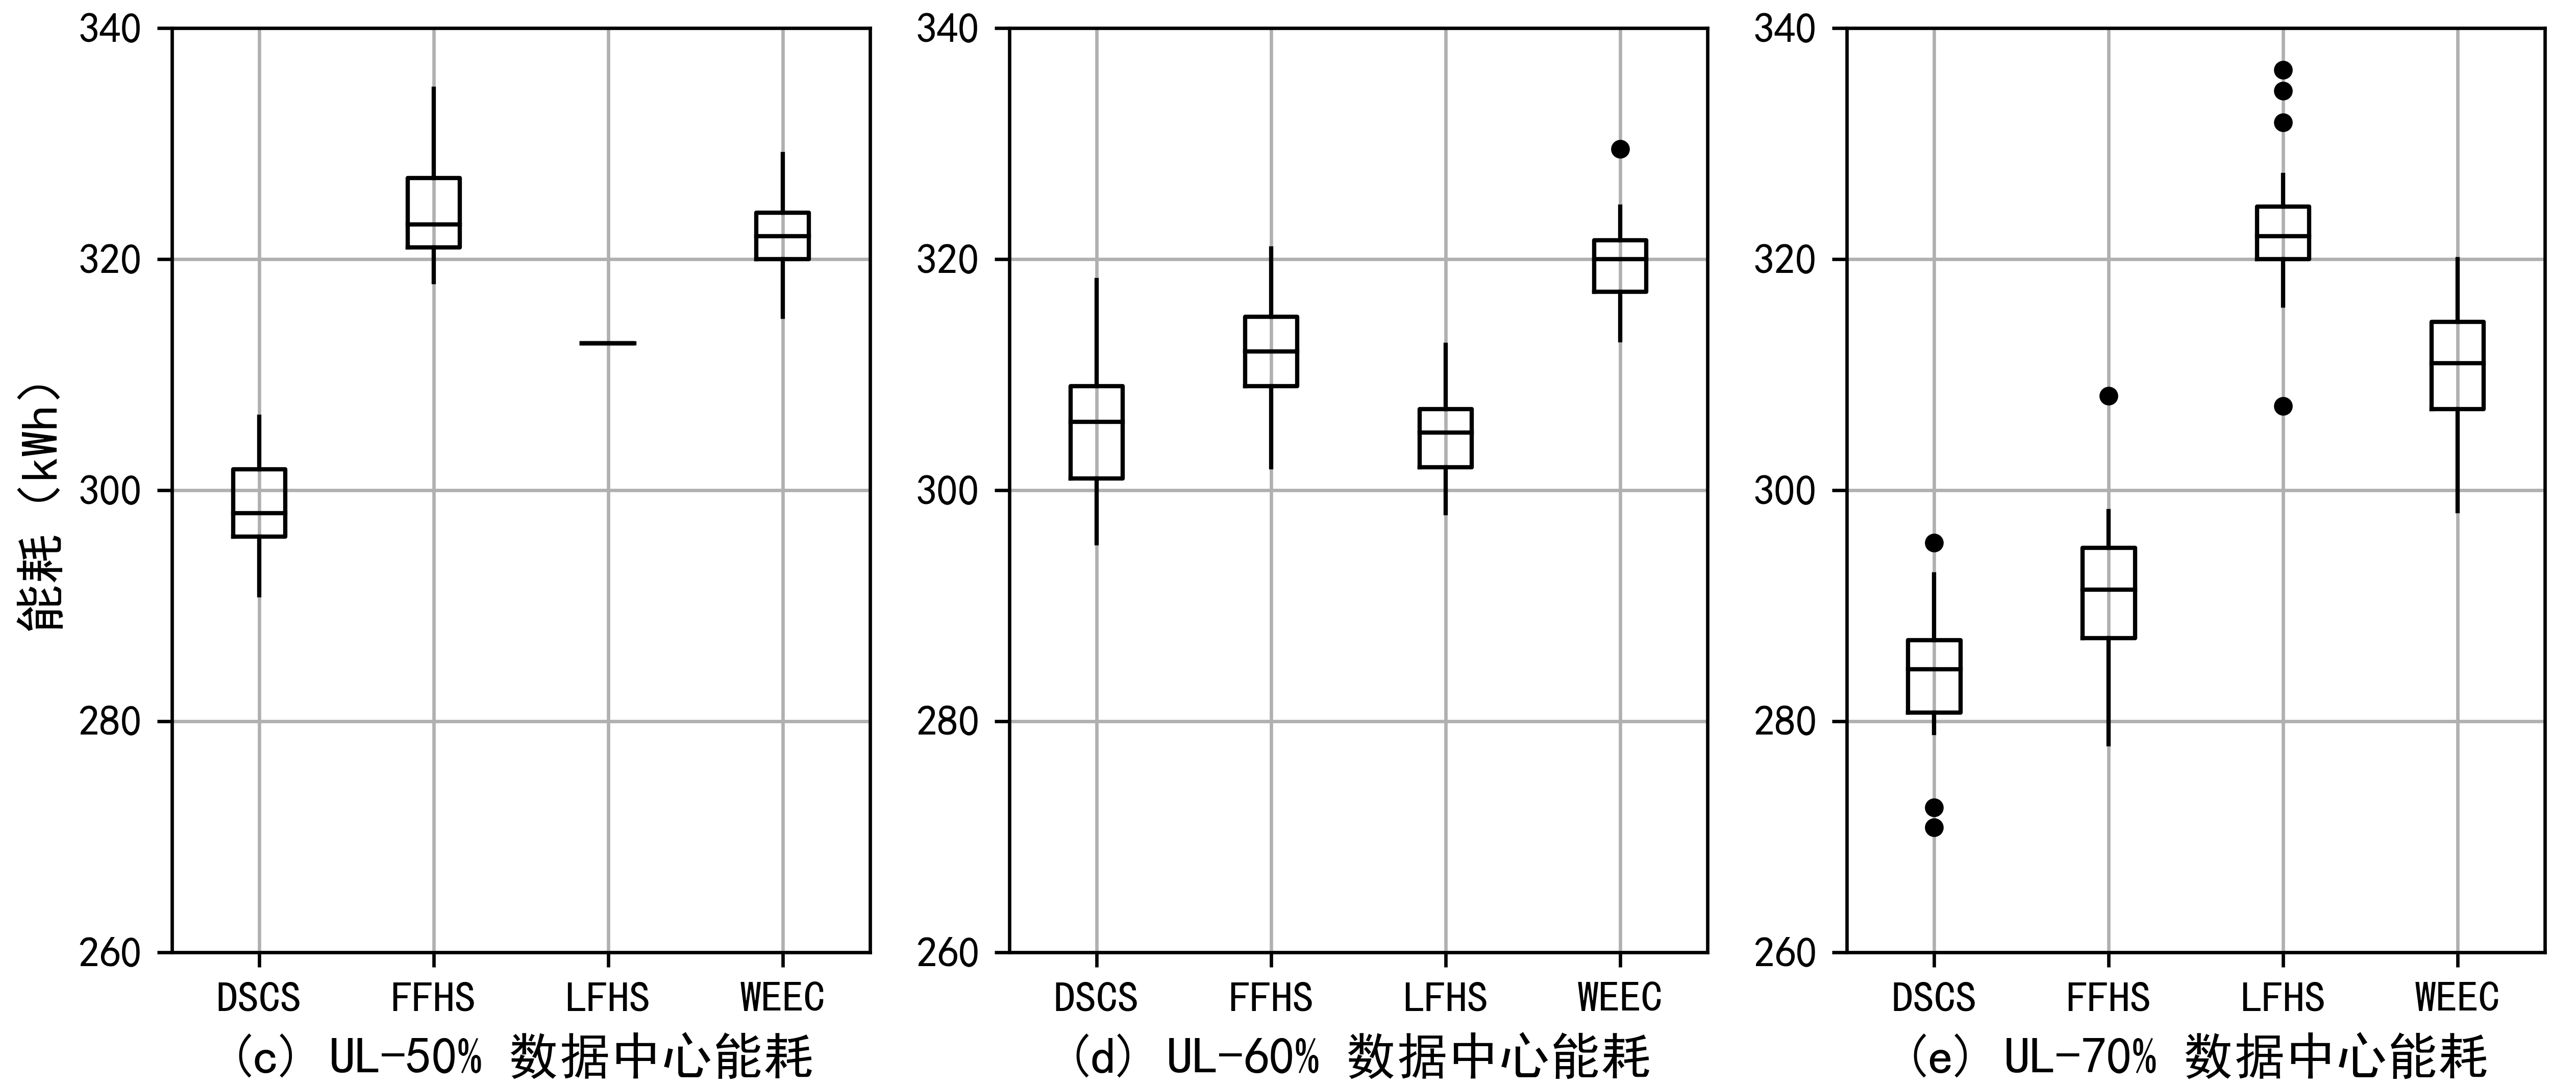
\includegraphics[width=0.45\textwidth]{figures/fig16_4-5_b.png}
    \end{figure}
\end{minipage}
\begin{minipage}{\textwidth}
    \centering
    \begin{figure}[htb]
    \centering
    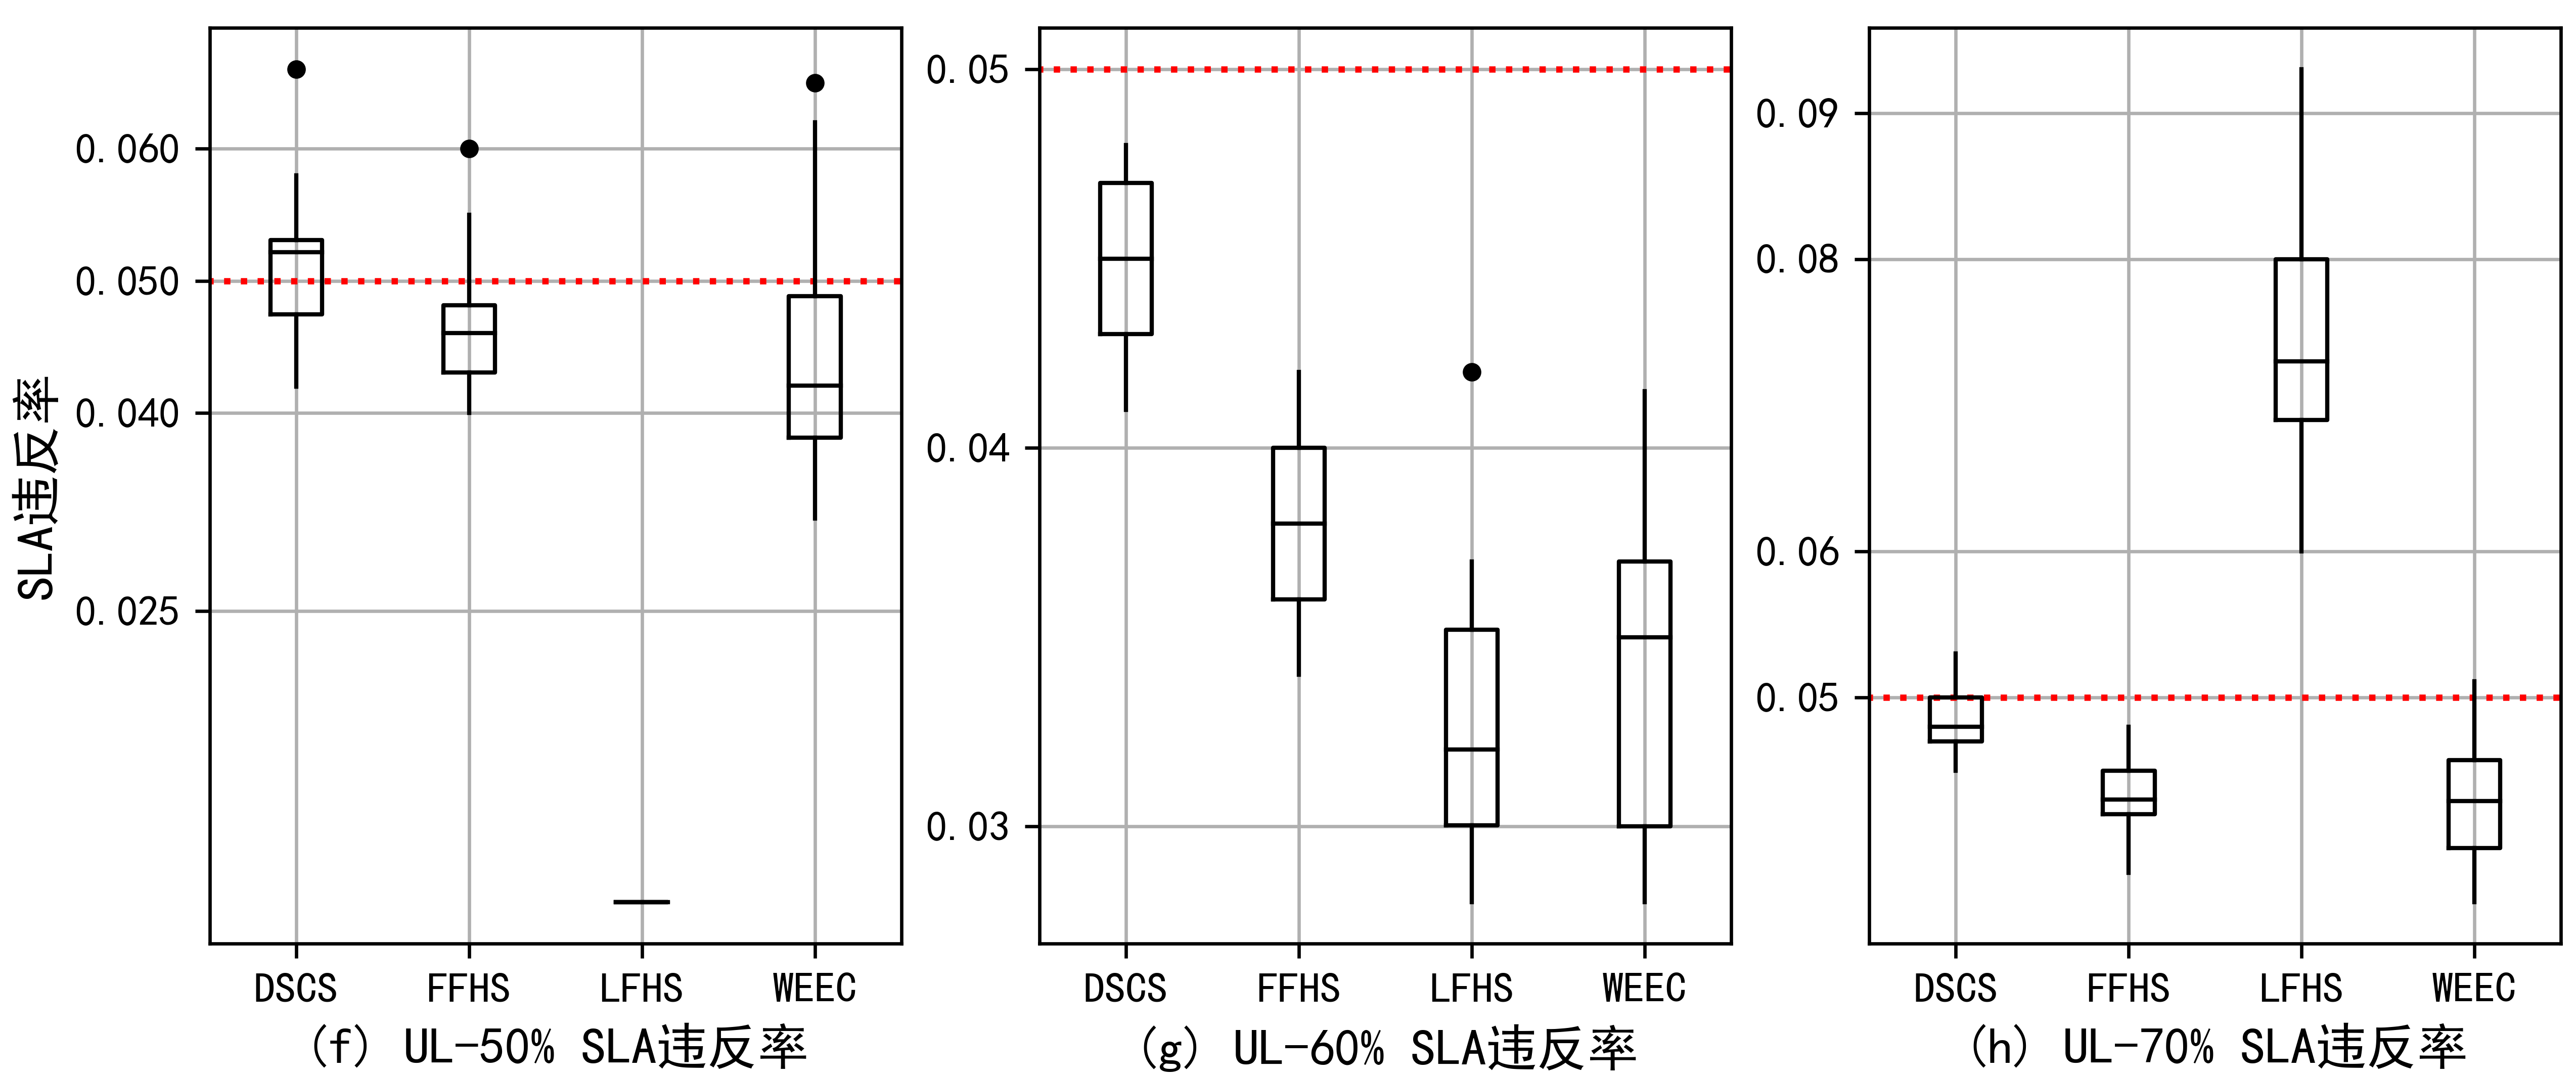
\includegraphics[width=0.45\textwidth]{figures/fig16_4-5_c.png}
    \caption{group.2 4种调度策略容器迁移、虚拟机创建数、能耗和SLA对比}
    \label{fig:fig16}
    \end{figure}
\end{minipage}
\end{frame}

\begin{frame}
\frametitle{实验结果与分析}
\framesubtitle{实验结果:group.3 \textbf{UL=$70\%$ OL=$80\%$, Overbooking=$[20th,40th,80th]$}}
\begin{minipage}{\textwidth}
    \centering
    \begin{figure}[htb]
    \centering
    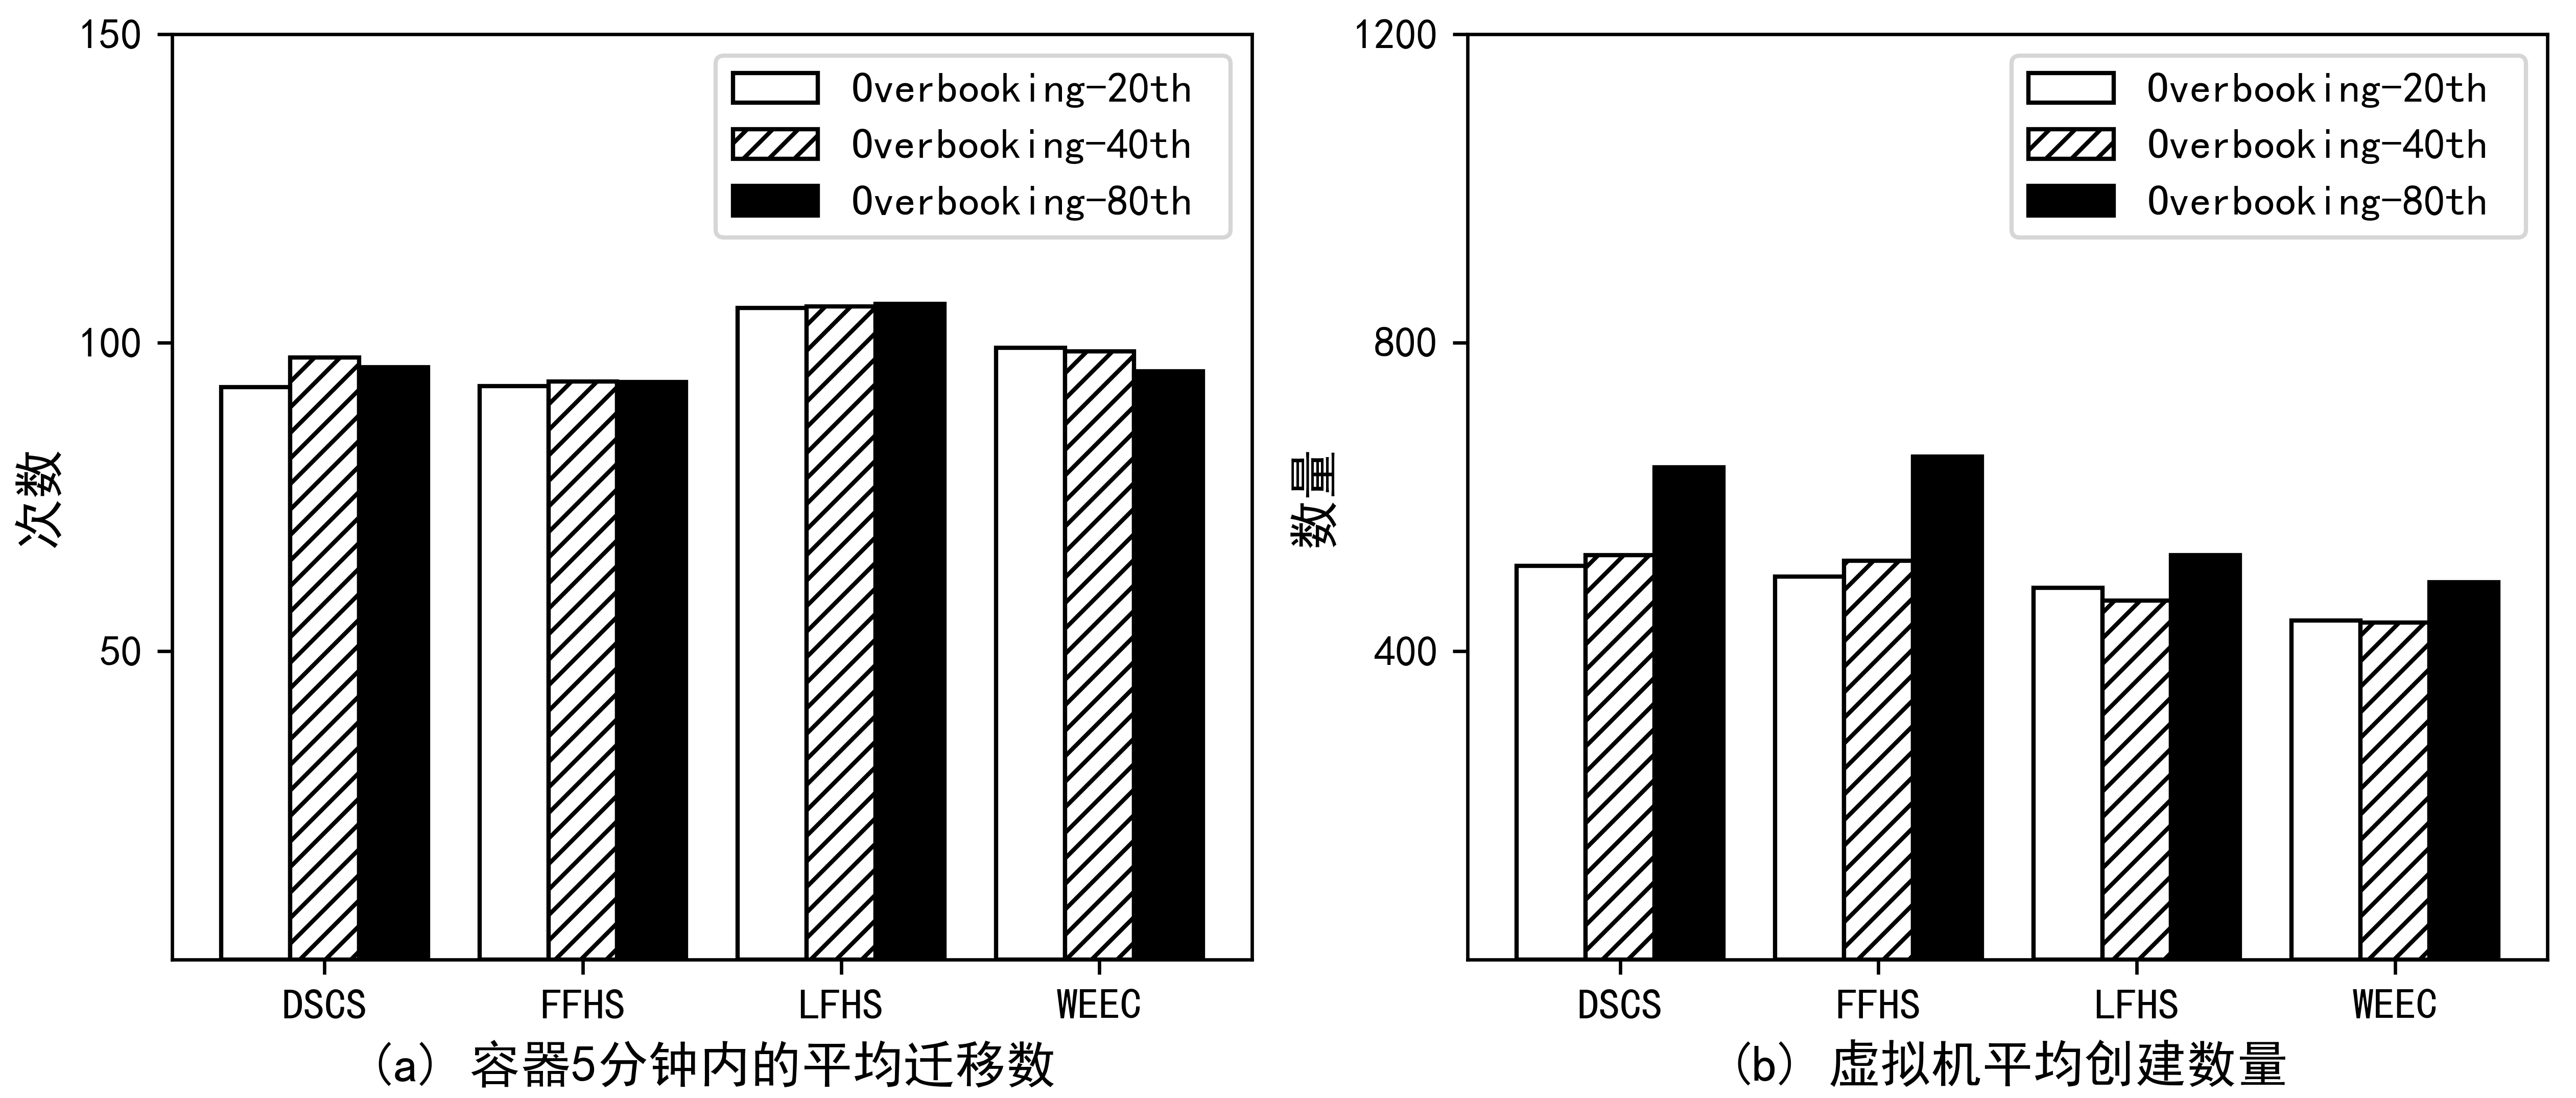
\includegraphics[width=0.45\textwidth]{figures/fig17_4-6_a.png}
    \end{figure}
\end{minipage}
\begin{minipage}{\textwidth}
    \centering
    \begin{figure}[htb]
    \centering
    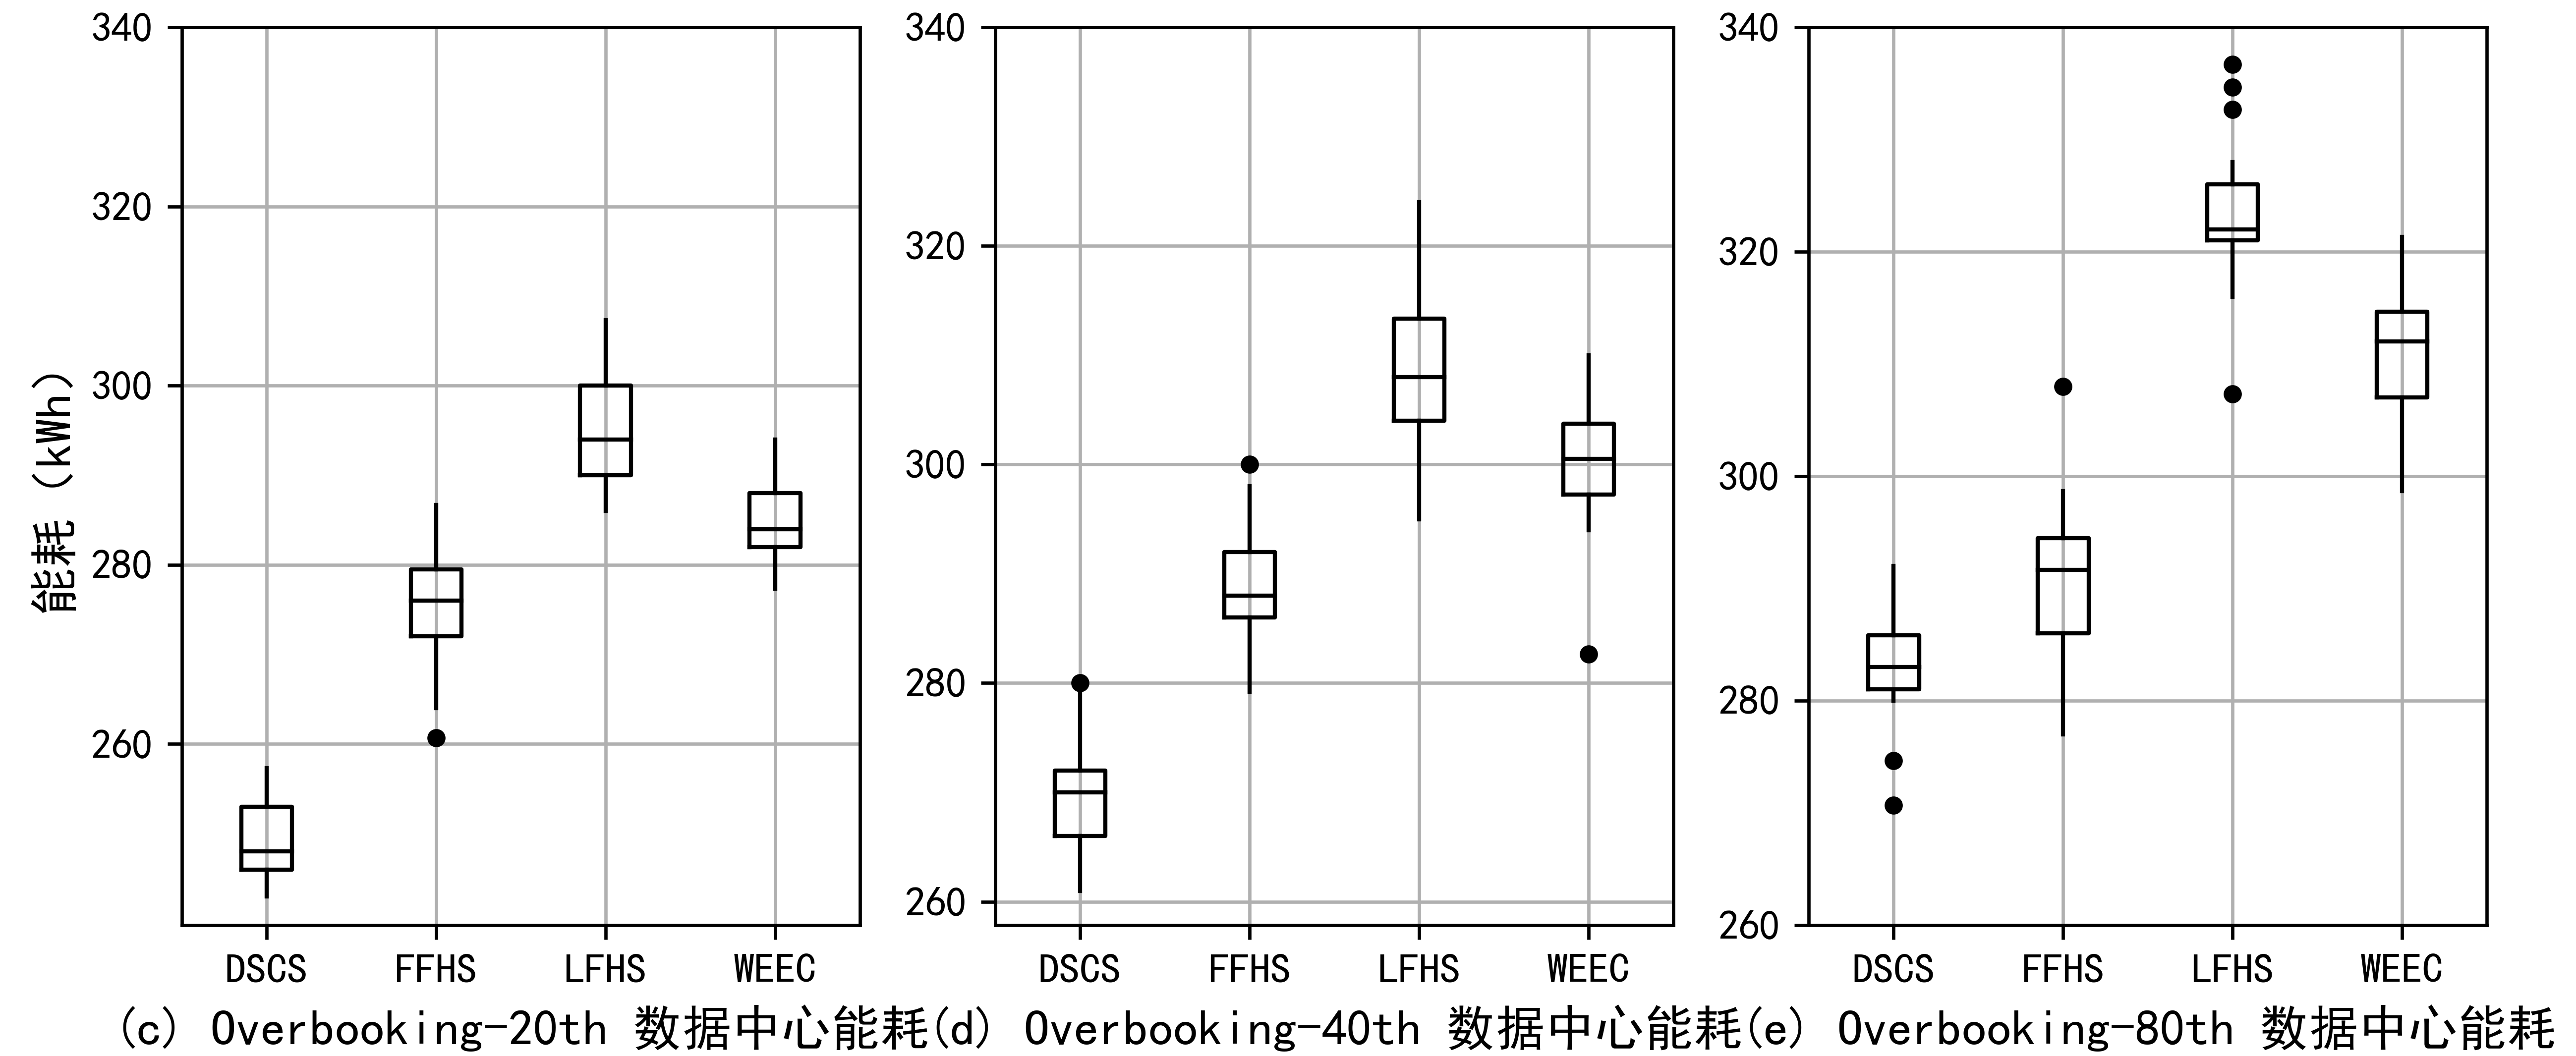
\includegraphics[width=0.45\textwidth]{figures/fig17_4-6_b.png}
    \end{figure}
\end{minipage}
\begin{minipage}{\textwidth}
    \centering
    \begin{figure}[htb]
    \centering
    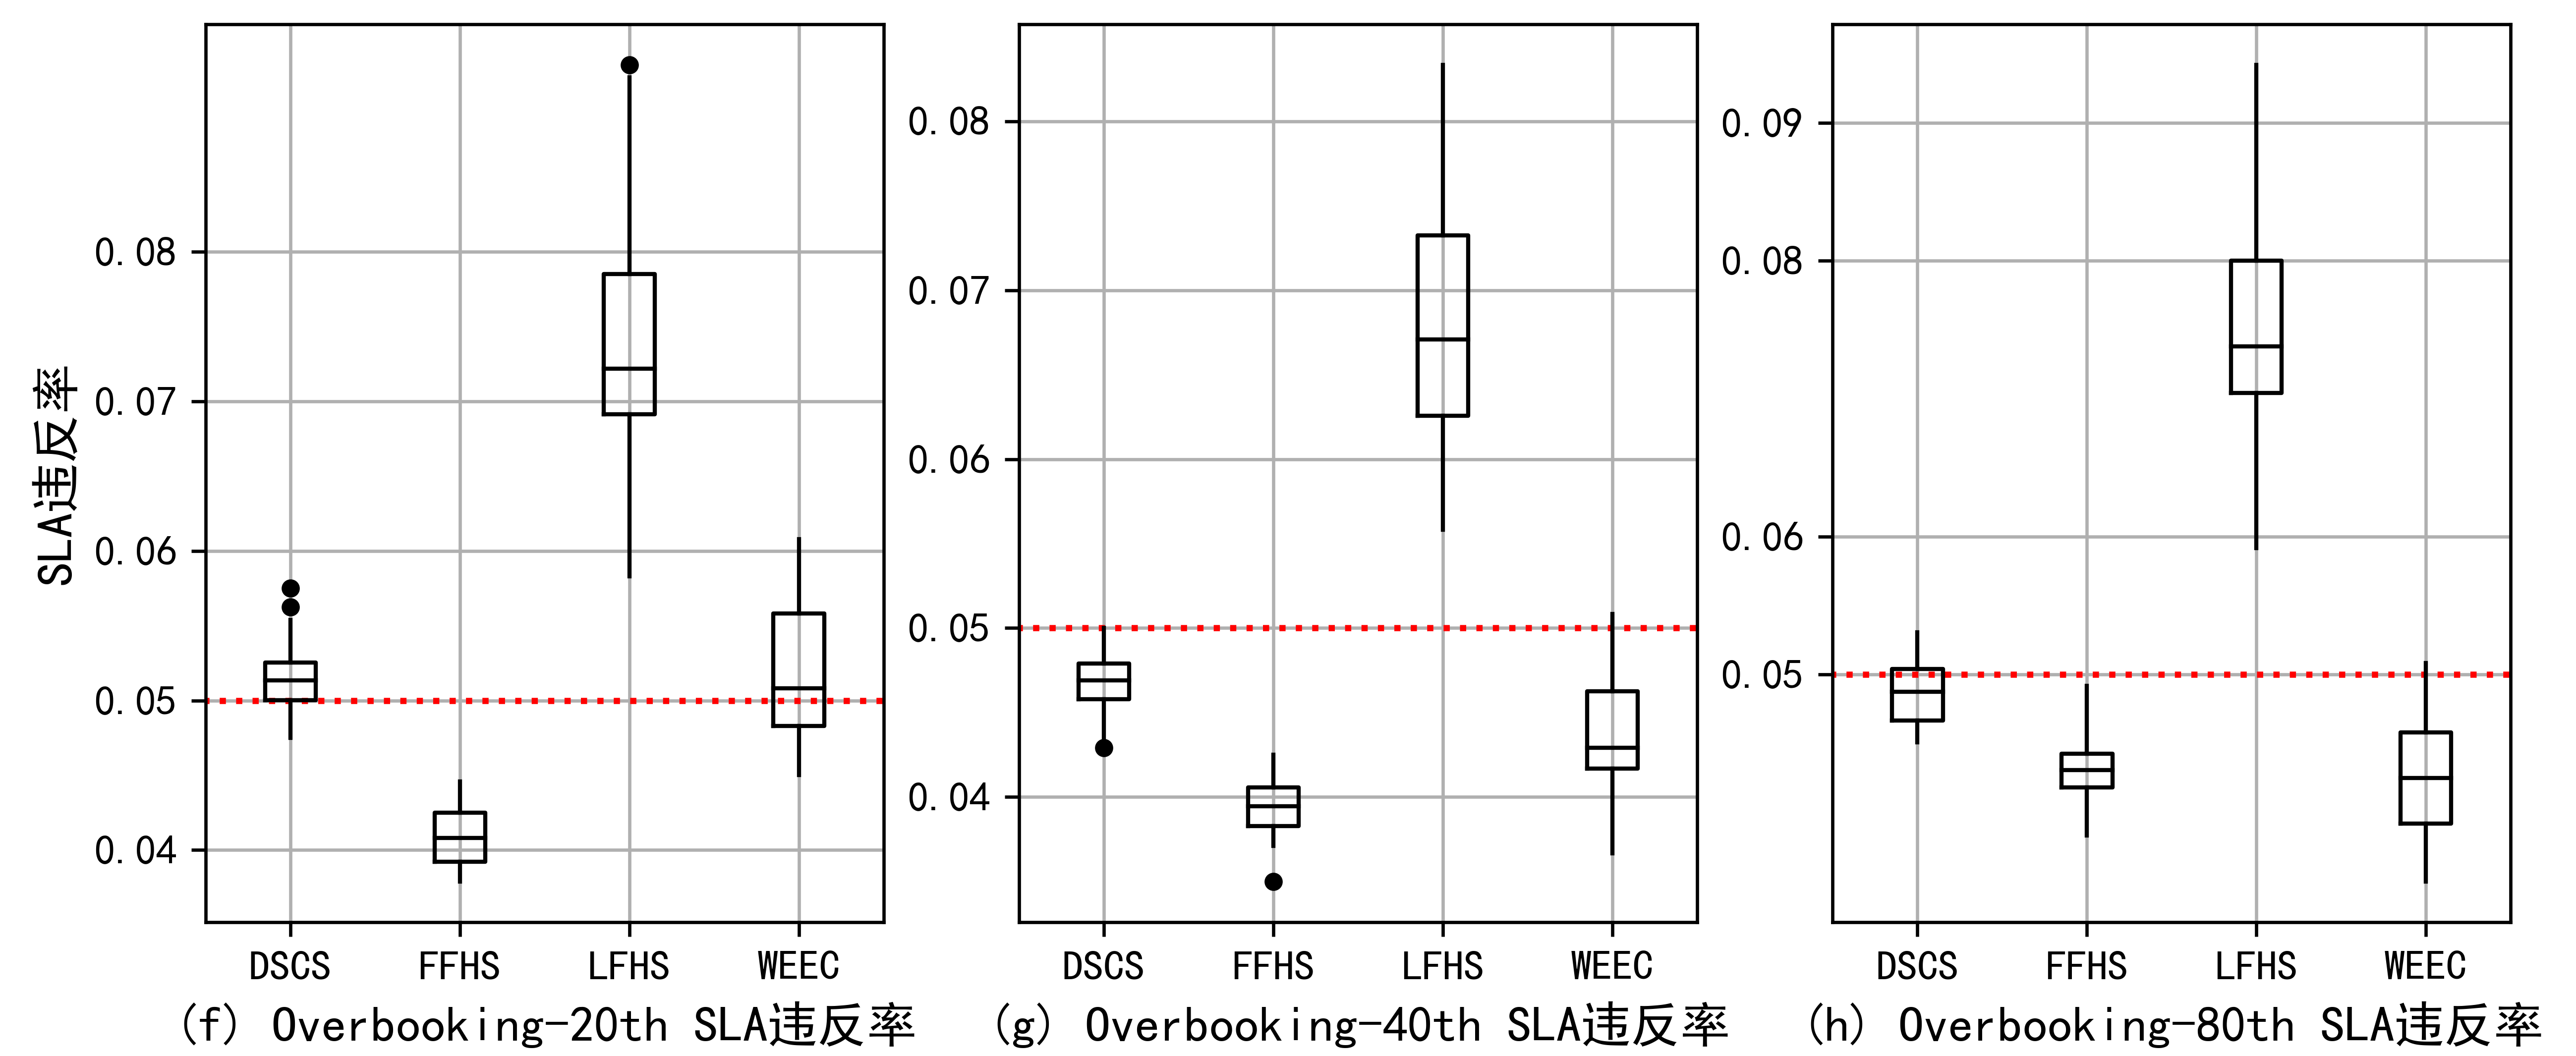
\includegraphics[width=0.45\textwidth]{figures/fig17_4-6_c.png}
    \caption{group.3 4种调度策略容器迁移、虚拟机创建数、能耗和SLA对比}
    \label{fig:fig17}
    \end{figure}
\end{minipage}
\end{frame}

\begin{frame}
\frametitle{实验结果与分析}
\framesubtitle{SLA违反补偿协议}
\begin{itemize}
    \item 主流云服务商(GCP\footnote{\tiny{https://cloud.google.com/}},
    AWS\footnote{\tiny{https://aws.amazon.com/}},阿里云\footnote{\tiny{https://cn.aliyun.com/}})SLA违反补偿协议
\end{itemize}
\begin{table}[hftb]
        \centering
        \resizebox{0.8\textwidth}{!}{%
            \begin{tabular}{ccccc}
                \toprule
                \textbf{赔偿(相对于租金比例)} & \textbf{SLA违反率(未响应时间占比)} \\
                \midrule
                $0$ & $0\sim5\%$   \\
                $5$ & $5\%\sim15\%$   \\
                $10$ & $15\%\sim20\%$   \\
                $20$ & $20\%\sim25\%$   \\
                $35$ & $25\%\sim30\%$   \\
                $55$ & $30\%\sim45\%$   \\
                $80$ & $45\%\sim50\%$   \\
                $100$ & $50\%$以上   \\
                \bottomrule
            \end{tabular}
        }
        \caption{主流云供应商SLA违反补偿金计算}
        \label{tab:tab6}
    \end{table}
\end{frame}

%Summary
%Title of section
\section{总结与展望}

\begin{frame}
\frametitle{总结与展望}
\end{frame}
\end{document}
